%% %%%%%%%%%%%%%%%%%%%%%%%%%%%%%%%%%%%%%%%%%%%%%%%%%
%% Template for a conference paper, prepared for the
%% Food and Resource Economics Department - IFAS
%% UNIVERSITY OF FLORIDA
%% %%%%%%%%%%%%%%%%%%%%%%%%%%%%%%%%%%%%%%%%%%%%%%%%%
%% Version 1.0 // November 2019
%% %%%%%%%%%%%%%%%%%%%%%%%%%%%%%%%%%%%%%%%%%%%%%%%%%
%% Ariel Soto-Caro
%%  - asotocaro@ufl.edu
%%  - arielsotocaro@gmail.com
%% %%%%%%%%%%%%%%%%%%%%%%%%%%%%%%%%%%%%%%%%%%%%%%%%%
\documentclass[11pt]{article}
\usepackage{UF_FRED_paper_style}
\usepackage{tabularx}
\usepackage{siunitx}
\usepackage{tipa}
\usepackage{textcmds}
\usepackage{multirow} 
%\usepackage{xcolor}
\usepackage[dvipsnames]{xcolor}
\usepackage{soul}
\definecolor{HLColor}{RGB}{230,230,250}
\sethlcolor{HLColor}
\usepackage[
    backend=biber,
    style=numeric,
  ]{biblatex}

\addbibresource{references.bib}
%% ===============================================
%% Setting the line spacing (3 options: only pick one)
%\doublespacing
% \singlespacing
\onehalfspacing
%% ===============================================
 
%\setlength{\droptitle}{-5em} %% Don't touch

% %%%%%%%%%%%%%%%%%%%%%%%%%%%%%%%%%%%%%%%%%%%%%%%%%%%%%%%%%%
% SET THE TITLE
% %%%%%%%%%%%%%%%%%%%%%%%%%%%%%%%%%%%%%%%%%%%%%%%%%%%%%%%%%%

% TITLE:
\title{\textbf{User Interface Design: Deliverable D2}\\Moodtracker for Companies}

% AUTHORS:
\author{Laurenz Kottek\\ Céline Nöhl\\ Alexandros Tsaparas\\ Noé Barbera}


    
% DATE:
\date{\today}

% %%%%%%%%%%%%%%%%%%%%%%%%%%%%%%%%%%%%%%%%%%%%%%%%%%%%%%%%%%
% %%%%%%%%%%%%%%%%%%%%%%%%%%%%%%%%%%%%%%%%%%%%%%%%%%%%%%%%%%
\begin{document}
% %%%%%%%%%%%%%%%%%%%%%%%%%%%%%%%%%%%%%%%%%%%%%%%%%%%%%%%%%%
% %%%%%%%%%%%%%%%%%%%%%%%%%%%%%%%%%%%%%%%%%%%%%%%%%%%%%%%%%%
% ABSTRACT
% %%%%%%%%%%%%%%%%%%%%%%%%%%%%%%%%%%%%%%%%%%%%%%%%%%%%%%%%%%
% %%%%%%%%%%%%%%%%%%%%%%%%%%%%%%%%%%%%%%%%%%%%%%%%%%%%%%%%%%
{\setstretch{.8}}
\maketitle 

\vspace{15mm}


\tableofcontents
\newpage


\section{Scenarios}

\subsection{Scenario 1}
Mr. Smith is a team leader in a Data Science company. The current project is about creating a new smartphone application. Therefore multiple teams are working together. He got bad feedback from some team members that they are not feeling good in the team. As he is very interested in the wellbeing of his team, he wants to improve the communication and the working climate between the teams. For this reason he uses the mood tracker app. In the app every employee has to answer some questions about the working conditions and has the option to give some direct feedback. After he received all the answered surveys he knows better about the mood of his employees. He sees that the developing team feels overwhelmed by all the designs the designing team has created. In the next team meeting he talks to the designing team and explains that they create designs that are too complicated and the developing team has a hard time implementing them. \\
After a couple of days the employees have to answer the next survey. There Mr. Smith sees that the developing team feels now more comfortable. 



\subsection{Scenario 2}
Jordan works for a pharmaceutical company. He works there in a team of 10 people. He hasn't been feeling well mentally for a few weeks. Since a few unpleasant things have happened in his family recently, this has put a strain on his everyday life. He notices that he is sometimes irritable and less productive at work. A few months ago, his company introduced a new tool for employee surveys. Employees are asked to regularly answer questions about their well-being and satisfaction with their working conditions. He truthfully answered the last survey rather poorly. As there were also a few questions about mental health, the app gave him some suggestions on how to deal with difficult situations. He was also given the option of talking to the company's therapist. As he didn't know anything about the therapist yet, he decided to speak to the therapist, Michael, after work. Not only that he realizes some improvements in his current mood and productivity but also the mood-tracking app makes him see that the daily mood of him and the feedback he gives changed to the better.

\subsection{Scenario 3}
Anna has been working in a medium-sized company for some time. While she is competent in her work, she has recently encountered difficulties with a colleague, Max. The collaboration has become increasingly tense, negatively impacting Anna's well-being and productivity.
One day, Anna decides to use the features of the company´s Wellbeing App to improve the situation. Here is how she utilizes the app:\\
1. Fill out a feedback form: 
Anna opens the app and navigates to a specific section that allows her to provide (anonymous) feedback. She fills out a brief form describing her feelings and the challenges in working with Max. This includes expressing her emotions and detailing specific incidents.\\
2. Access additional support through management: 
As part of the feedback process, Anna has the option to escalate her concerns to management. The app provides a secure channel for her to share her feedback with relevant personnel in a confidential manner. This additional support ensures that someone in the management is aware of the problem and can intervene if necessary.\\
Through using the wellbeing application Anna´s mood and the working relationship with Max have improved a lot, so Anna is happy in her workplace again and does not encounter any big problems with Max recently. 

\subsection{Scenario 4}
Alice is a CEO for a company specialized in tech. Bob is a project manager in Alice’s company, and he is in charge of a team on a product, and he has noticed that recently, the productivity of the group and the quality of the results are decreasing, which is not a good sign for the future. Oscar is an employee and a member of Bob’s team, and he recently told Bob in a weekly meeting with the team that they weren’t feeling the best while working on this project. Bob, who is concerned about the well-being of his team and the advancement of the project, decides to set up a mood tracker in the team, where every member will give feedback daily and tell how they feel about certain subjects. Over the next weeks, Bob and Alice can analyze the data they get from the forms and feedback from the members of the team. With this, they can get conclusions about the mood of the team and spot the different problems there are and find solutions to them.
\clearpage

\section{Storyboards}
\subsection{Storyboard 1}
\begin{figure}[!h]
    \centering
    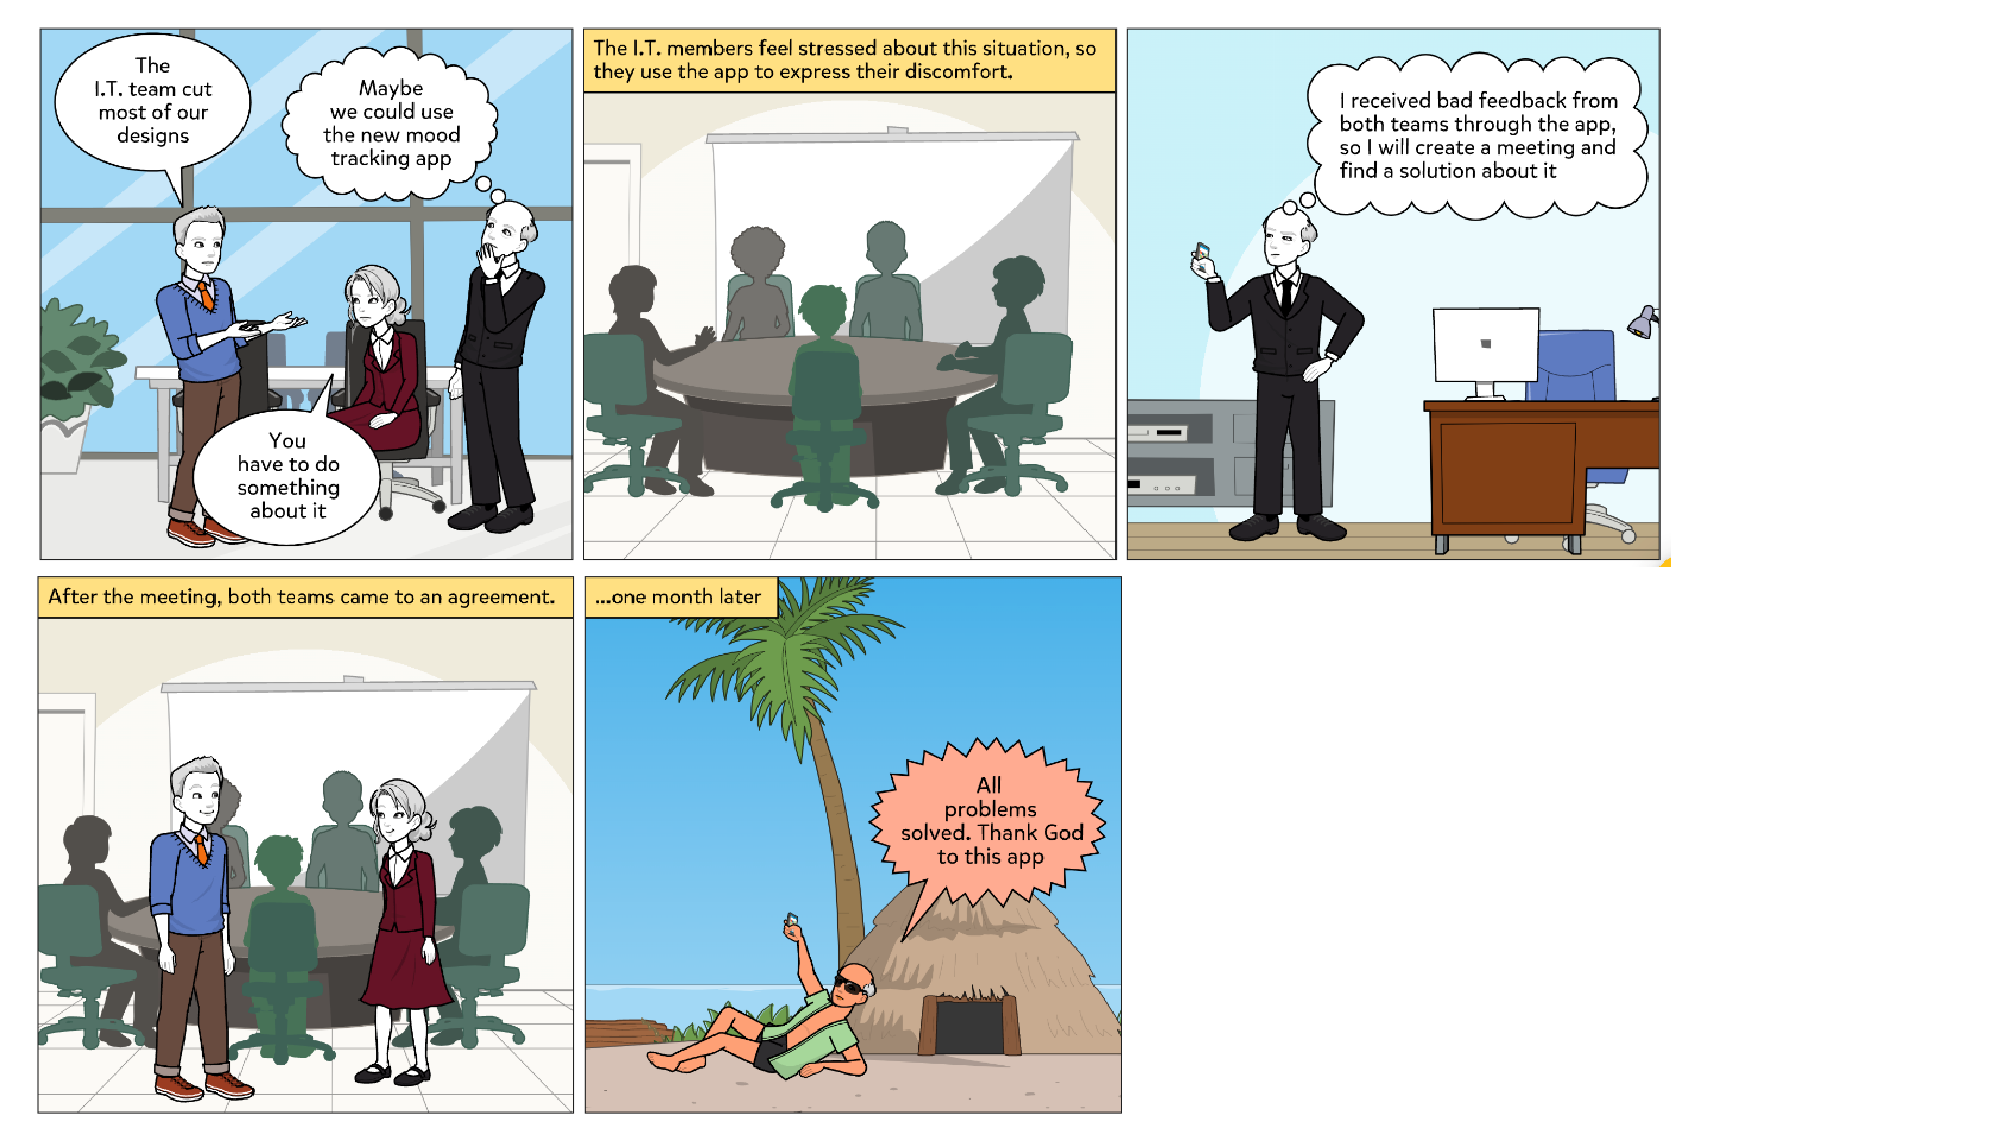
\includegraphics[scale = 0.5]{figures/Storyboard all.pdf}
\end{figure}
\subsection{Storyboard 2}
\begin{figure}[!h]
    \centering
    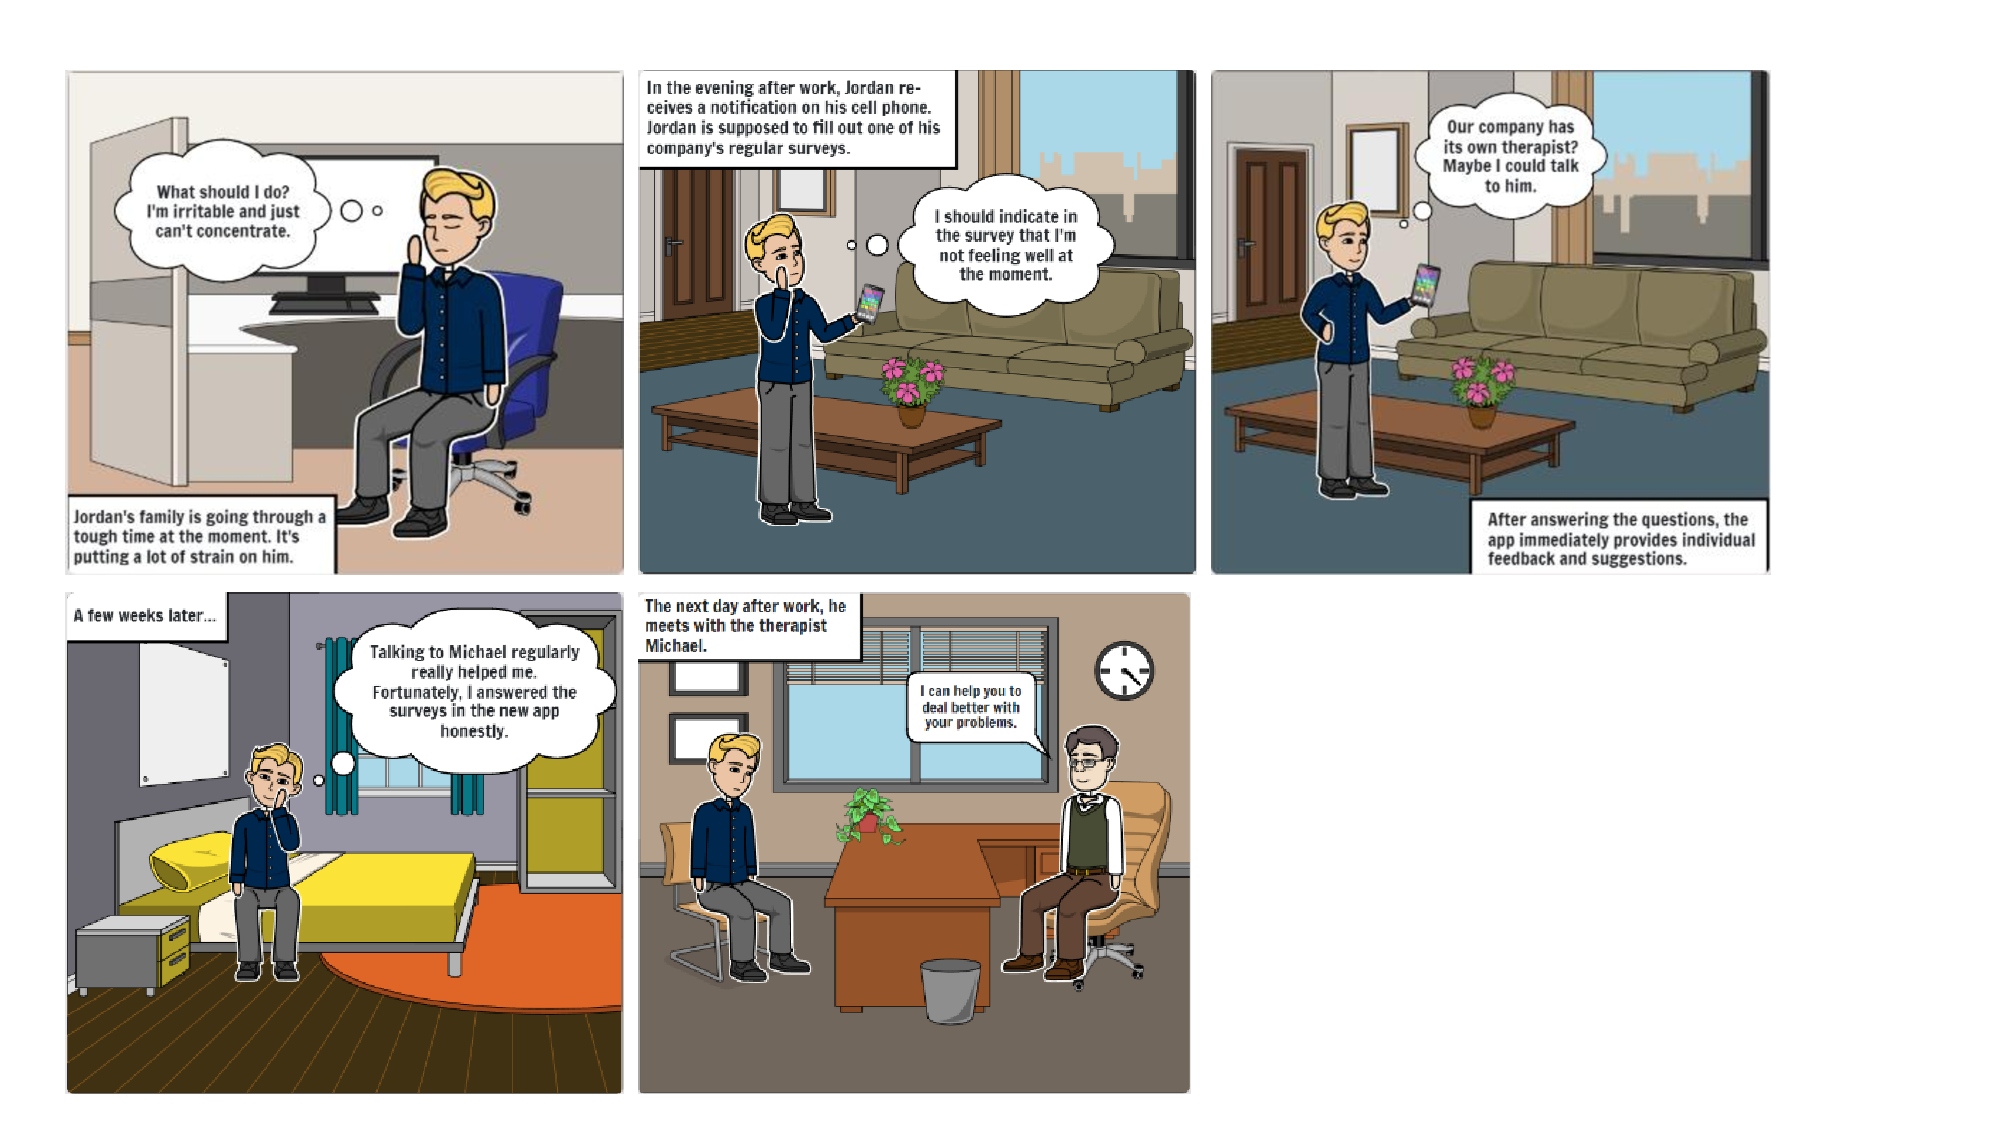
\includegraphics[scale = 0.5]{figures/Storyboard ich.pdf}
\end{figure}

\subsection{Storyboard 3}
\begin{figure}[!h]
    \centering
    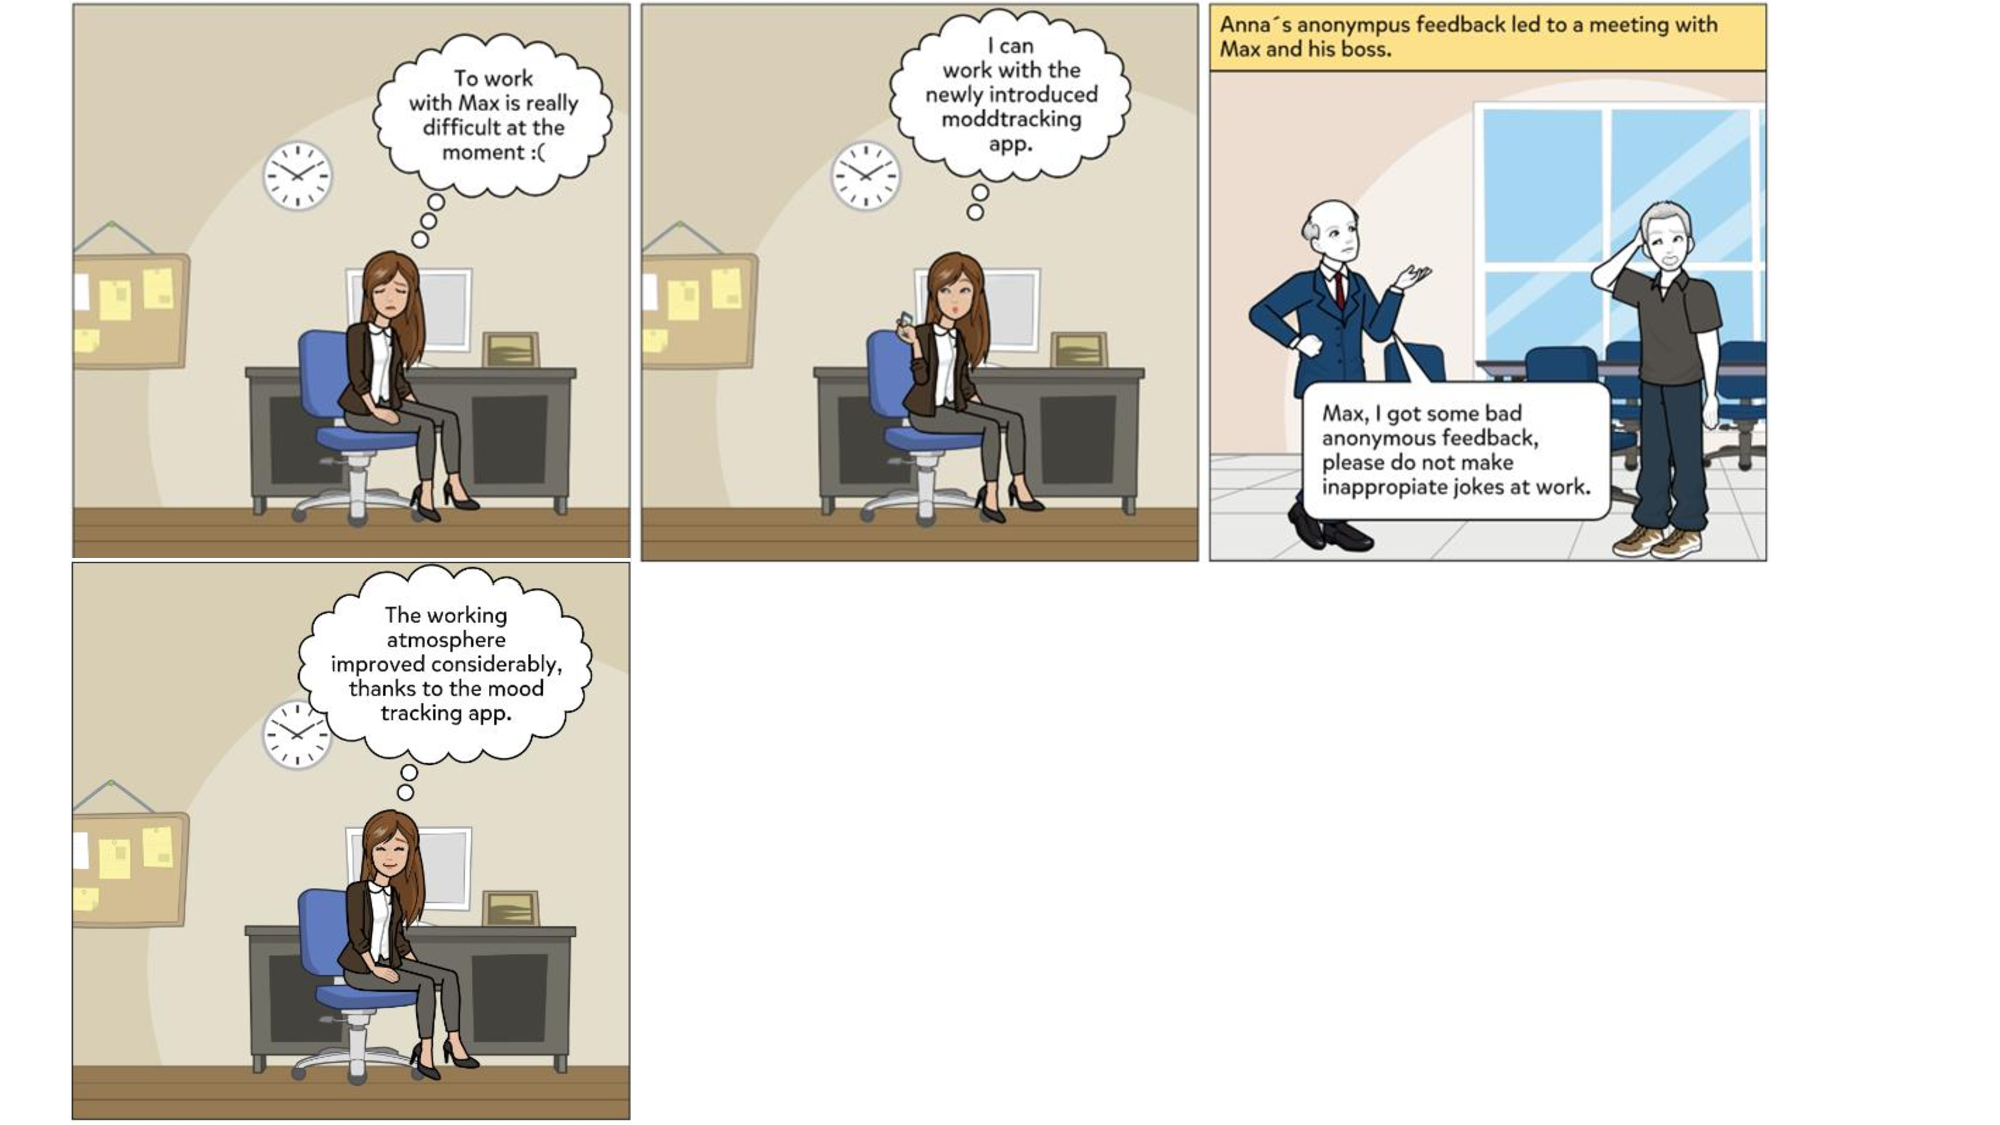
\includegraphics[scale = 0.5]{figures/Storyboard Laurenz.pdf}
\end{figure}

\clearpage

\section{Hierarchical Task Analysis}
\begin{figure}[!h]
    \centering
    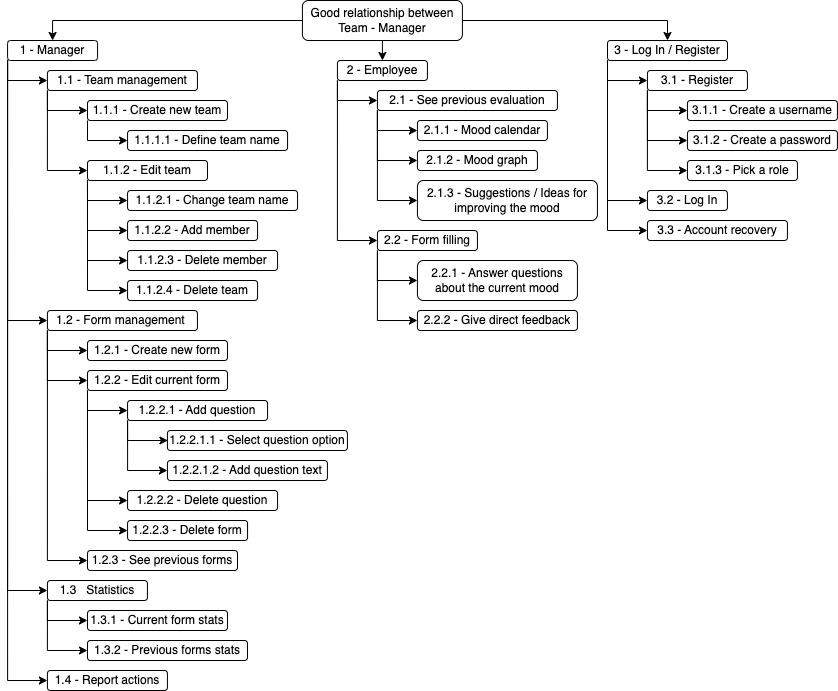
\includegraphics[scale = 0.5]{figures/HTA.png}
\end{figure}


\paragraph{Plan 1:}\mbox{}\\
Create a new survey: 1.2.1 $\rightarrow$ 1.2.2.1.1 $\rightarrow$ 1.2.2.1.2\\
See the results of the survey: 1.3.1 (latest survey) or 1.3.2 (previous surveys) \\ \hspace*{50mm}  $\rightarrow$ if action has been done, do 1.4\\
Create a new team: 1.1.1.1 $\rightarrow$ 1.1.2.2 
 
\paragraph{Plan 2:}\mbox{}\\
Answer the survey: 2.2.1 $\rightarrow$ optional: 2.2.2\\
Get suggestions to improve the mood: 2.1.3

\paragraph{Plan 3:}\mbox{}\\
Log in: If there is already an account, do 3.2, else: 3.1.1 $\rightarrow$ 3.1.2 $\rightarrow$ 3.1.3 

\newpage

\section{Paper Mockups}

\subsection{Design Studio}
We used the Design Studio technique for the paper mockups. In this way, we wanted to bring together initial design ideas and stimulate an initial exchange about the structure of our app. The process involved a total of two rounds, each consisting of a drawing phase, a presentation phase and a critique phase. The drawings in the first phase were intended to cover the basic functions of the app and include examples of team members and team managers. It was clear from the beginning that our application would be designed for smartphones.
\subsubsection{First Round}
The results of the first round for all team members are shown below.
\begin{figure}[!h]
    \centering
    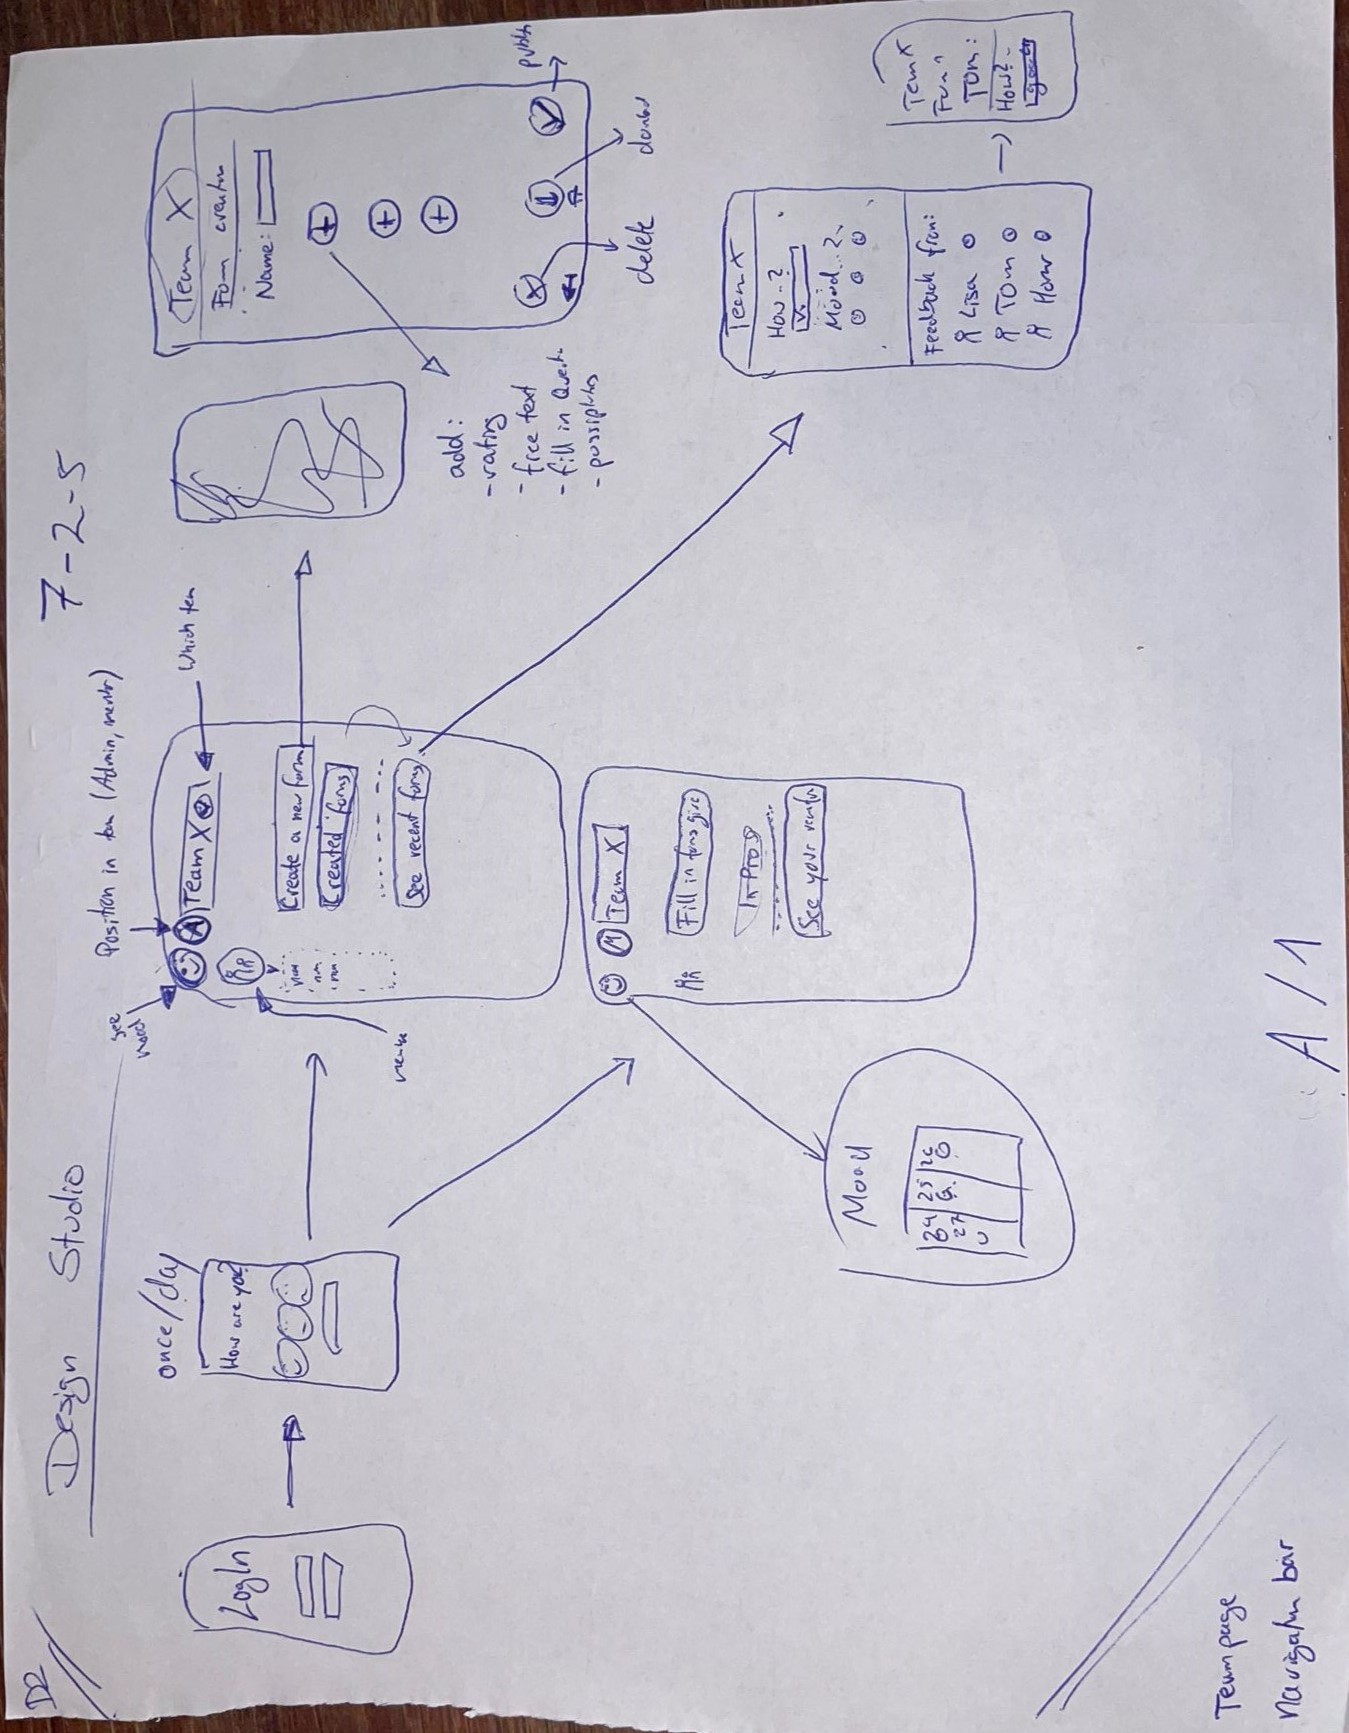
\includegraphics[scale = 0.3]{figures/A1.jpg}
    \caption{For team member A, the start screen is always the overview of the last team viewed. From there, you can switch to another team, take action in the team itself, or view a calendar overview with the progress of your own mood.}
\end{figure}

\begin{figure}[!h]
    \centering
    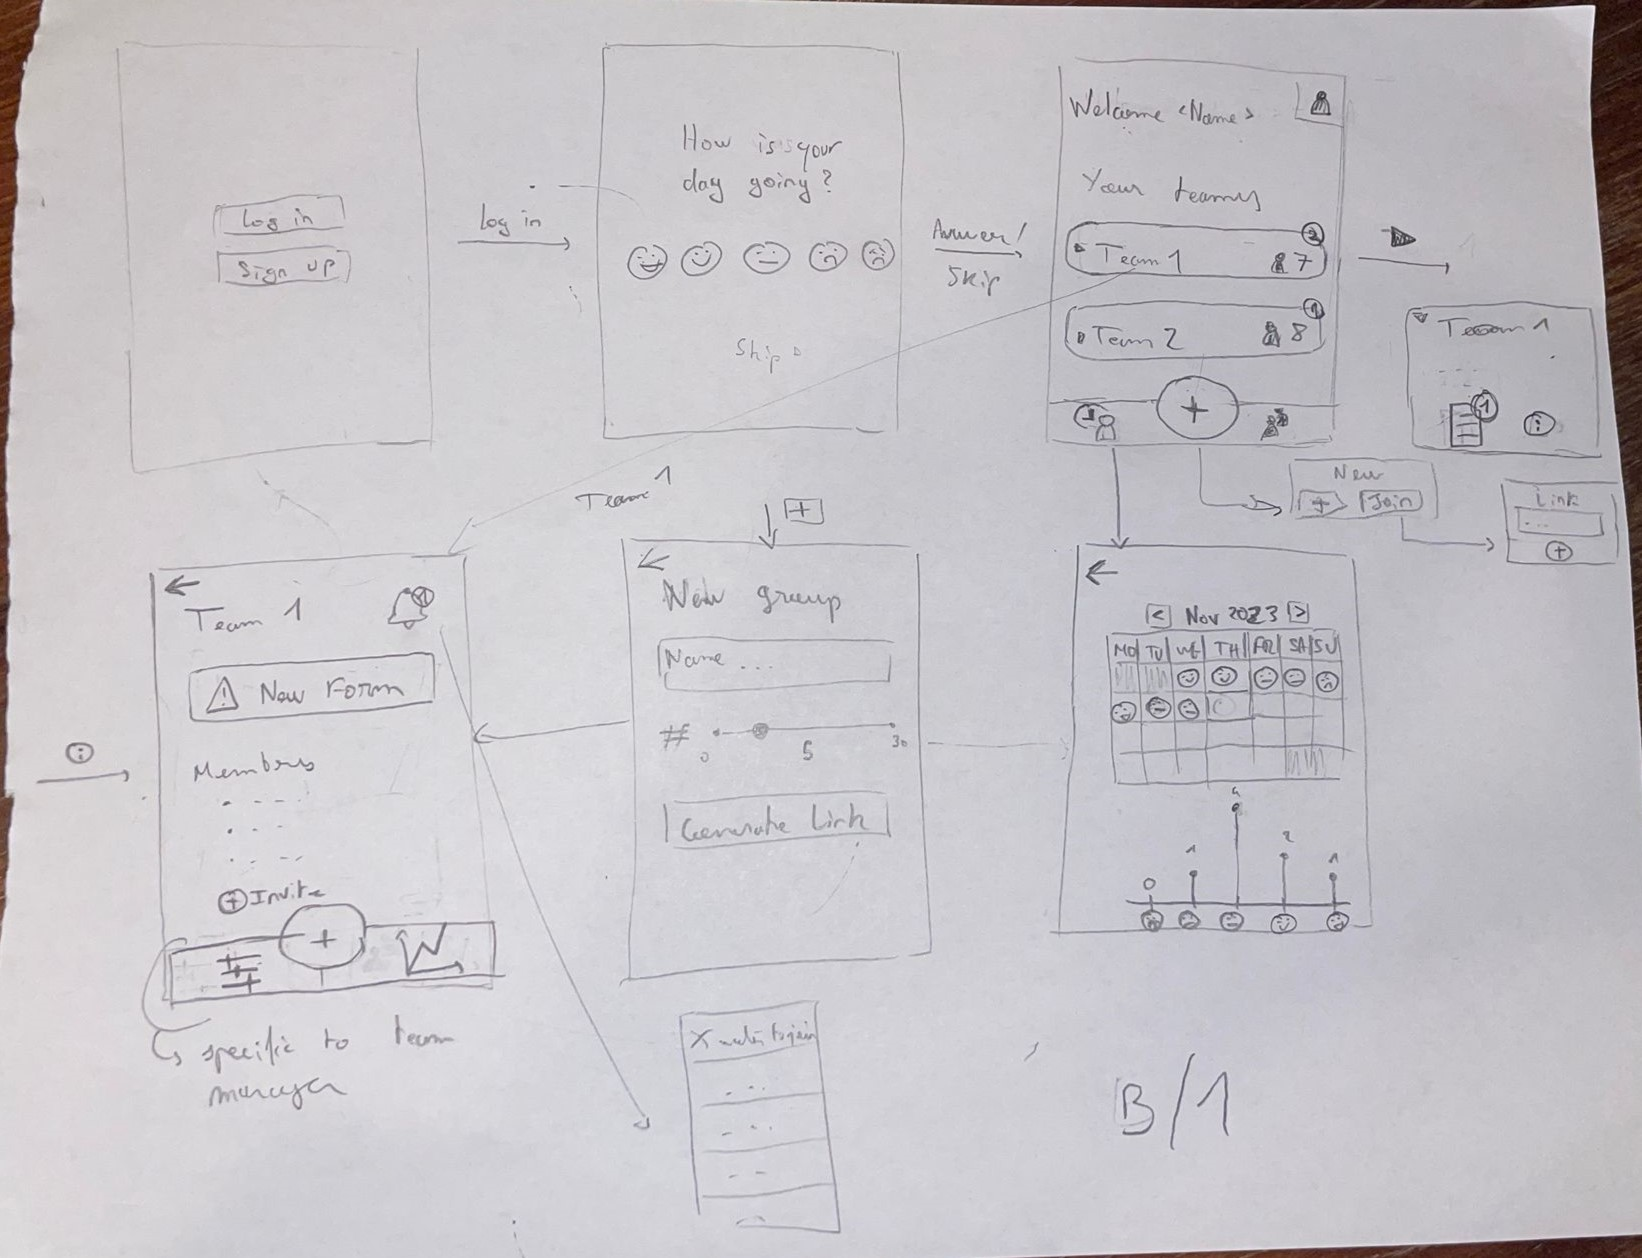
\includegraphics[scale = 0.45,angle=90]{figures/B1.jpg}
    \caption{Team member B had a new idea for the main screen in the first round, in which the teams are displayed similar to a chat list. In addition, the possibility has been created here to join teams yourself as a team member using an invitation link.}
\end{figure}
\clearpage

\begin{figure}[!h]
    \centering
    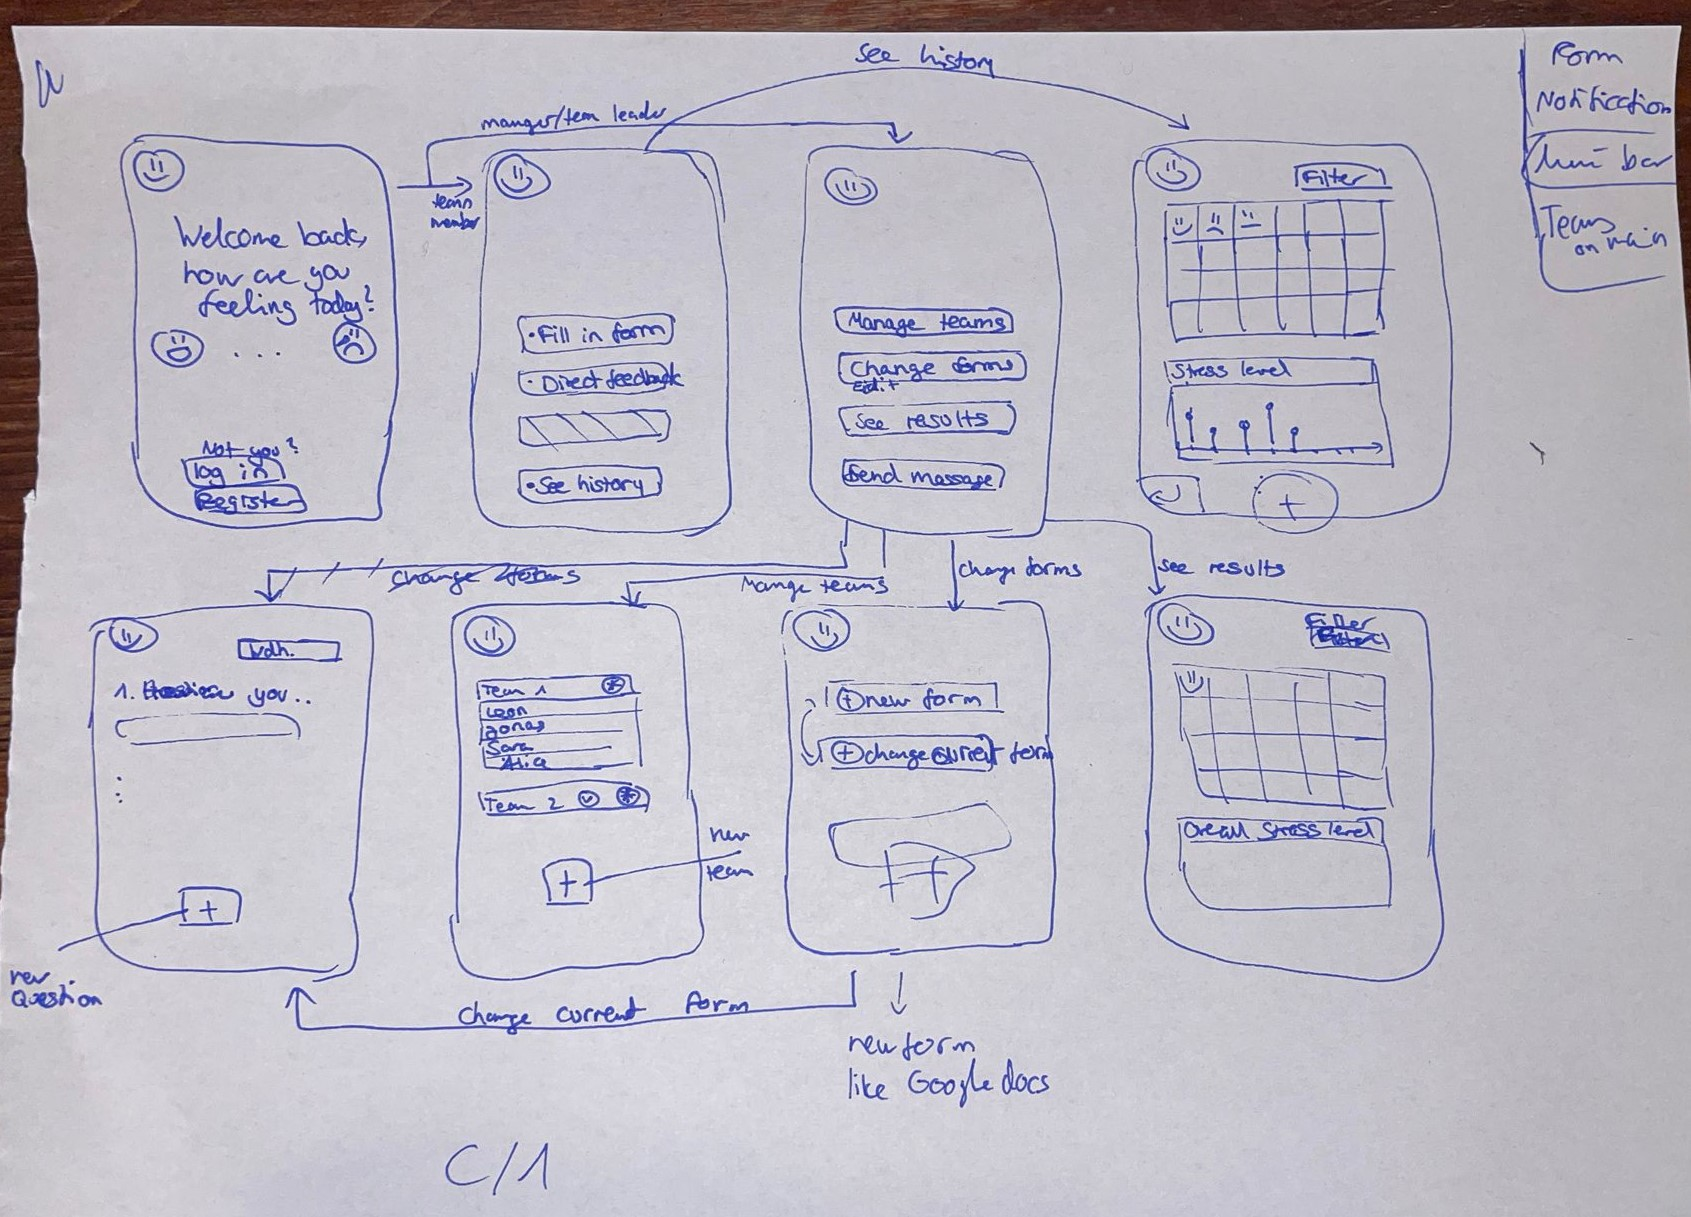
\includegraphics[scale = 0.45,angle=90]{figures/C1.jpg}
    \caption{With team member C, the arrangement of the teams is similar to that of A.}
\end{figure}

\begin{figure}[!h]
    \centering
    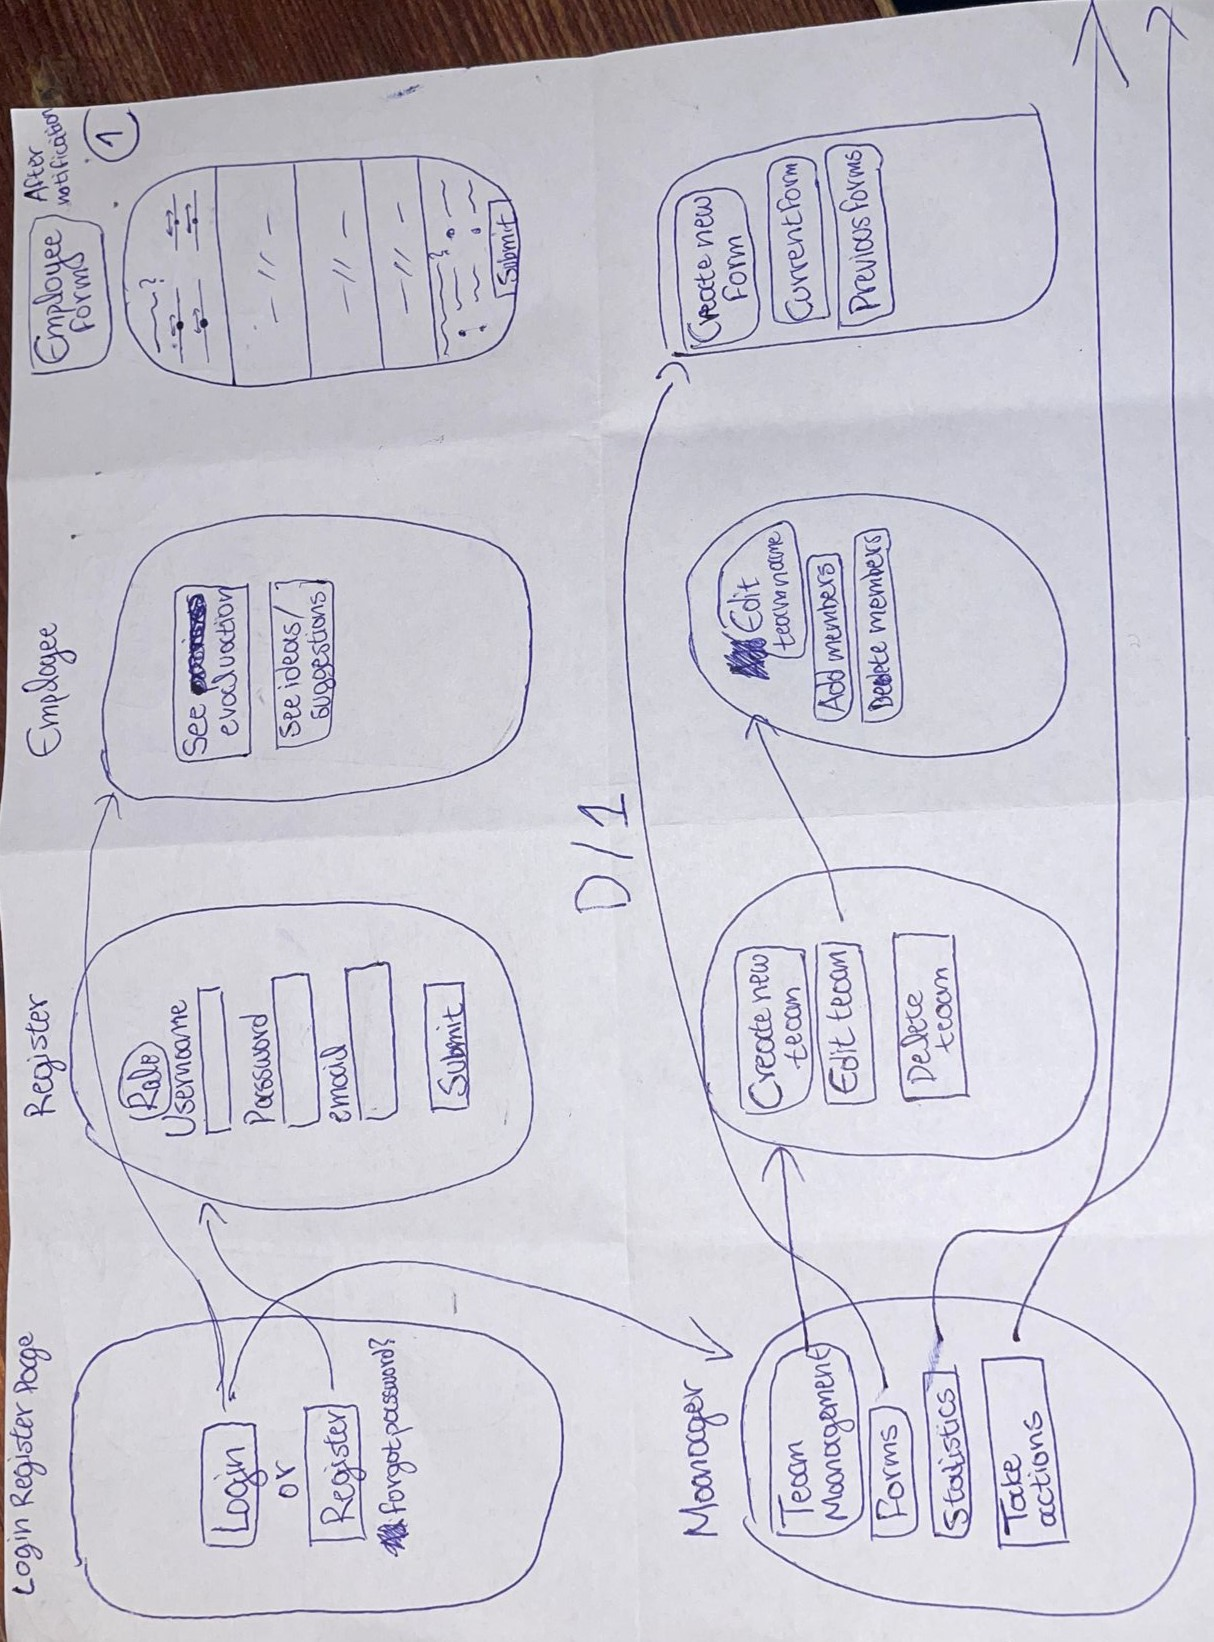
\includegraphics[width = \textwidth]{figures/D1.jpg}
    \caption{Team member D focused more on the functionality of the app than on the design, which is why the design elements were neglected here.}
\end{figure}

\begin{figure}[!h]
    \centering
    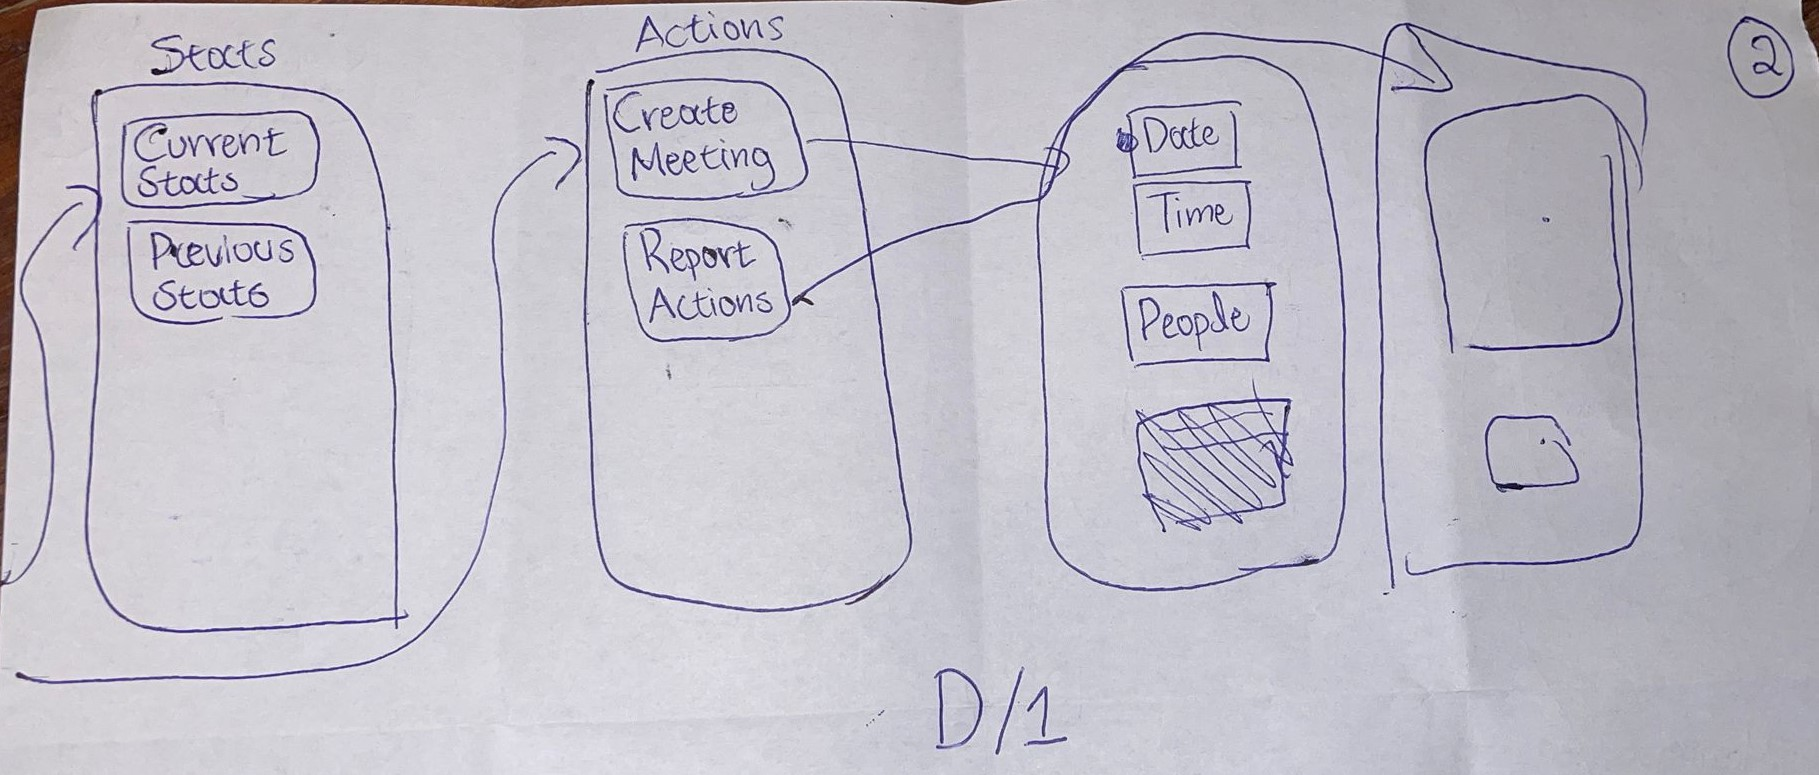
\includegraphics[width = \textwidth]{figures/D1.1.jpg}
    \caption{Second page of the solution from team member D.}
\end{figure}

\clearpage

\subsubsection{Second Round}
In the second round, you could quickly see that our results had evened out. Especially in the team overview, we all have a very similar solution in our mockups. The calendar view can also be found in 3 of the 4 designs. For Team Member B, the second round only has two screens, as changes were made to the design of the first round and these two screens were merely added.

\begin{figure}[!h]
    \centering
    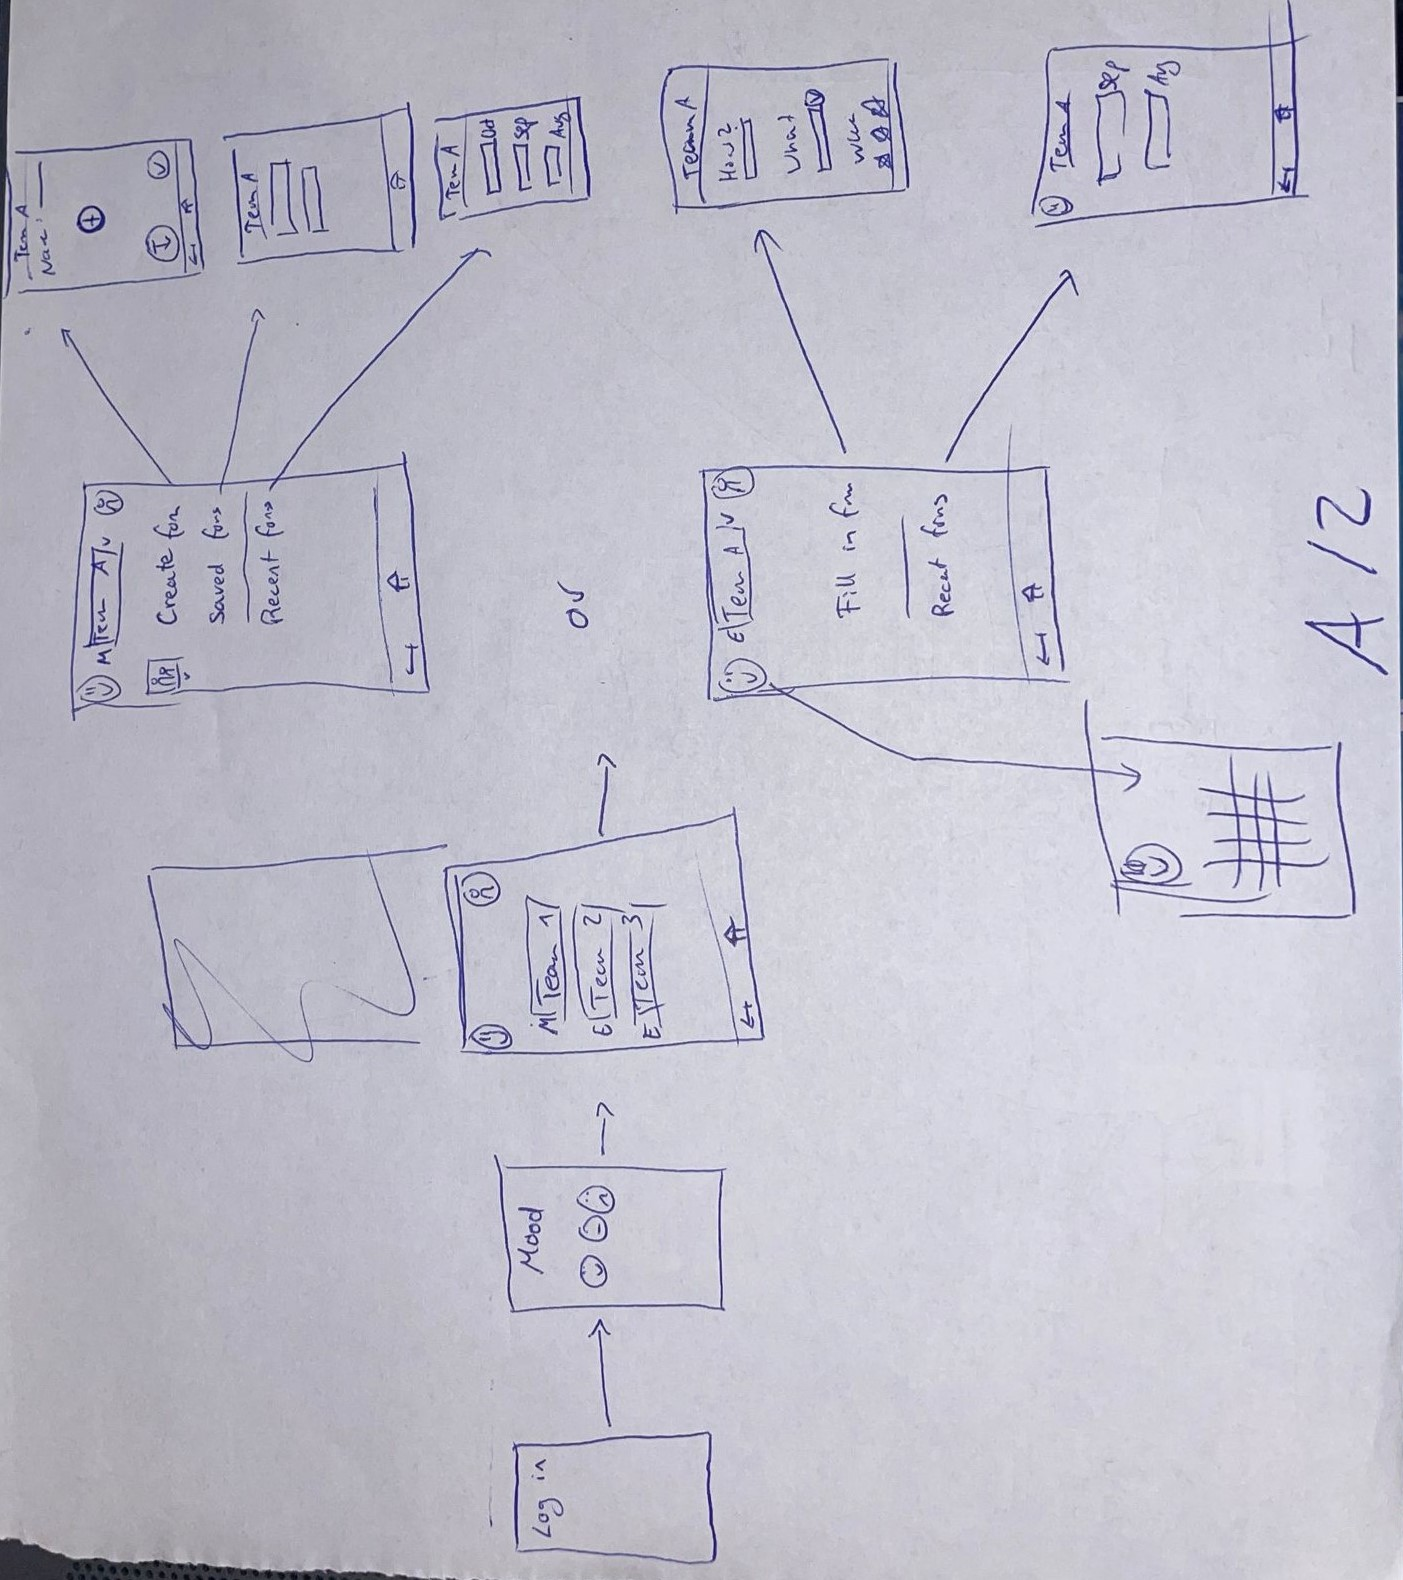
\includegraphics[scale=0.4]{figures/A2.jpg}
    \caption{In the second round, A adopted the main screen with the team overview.}
\end{figure}

\begin{figure}[!h]
    \centering
    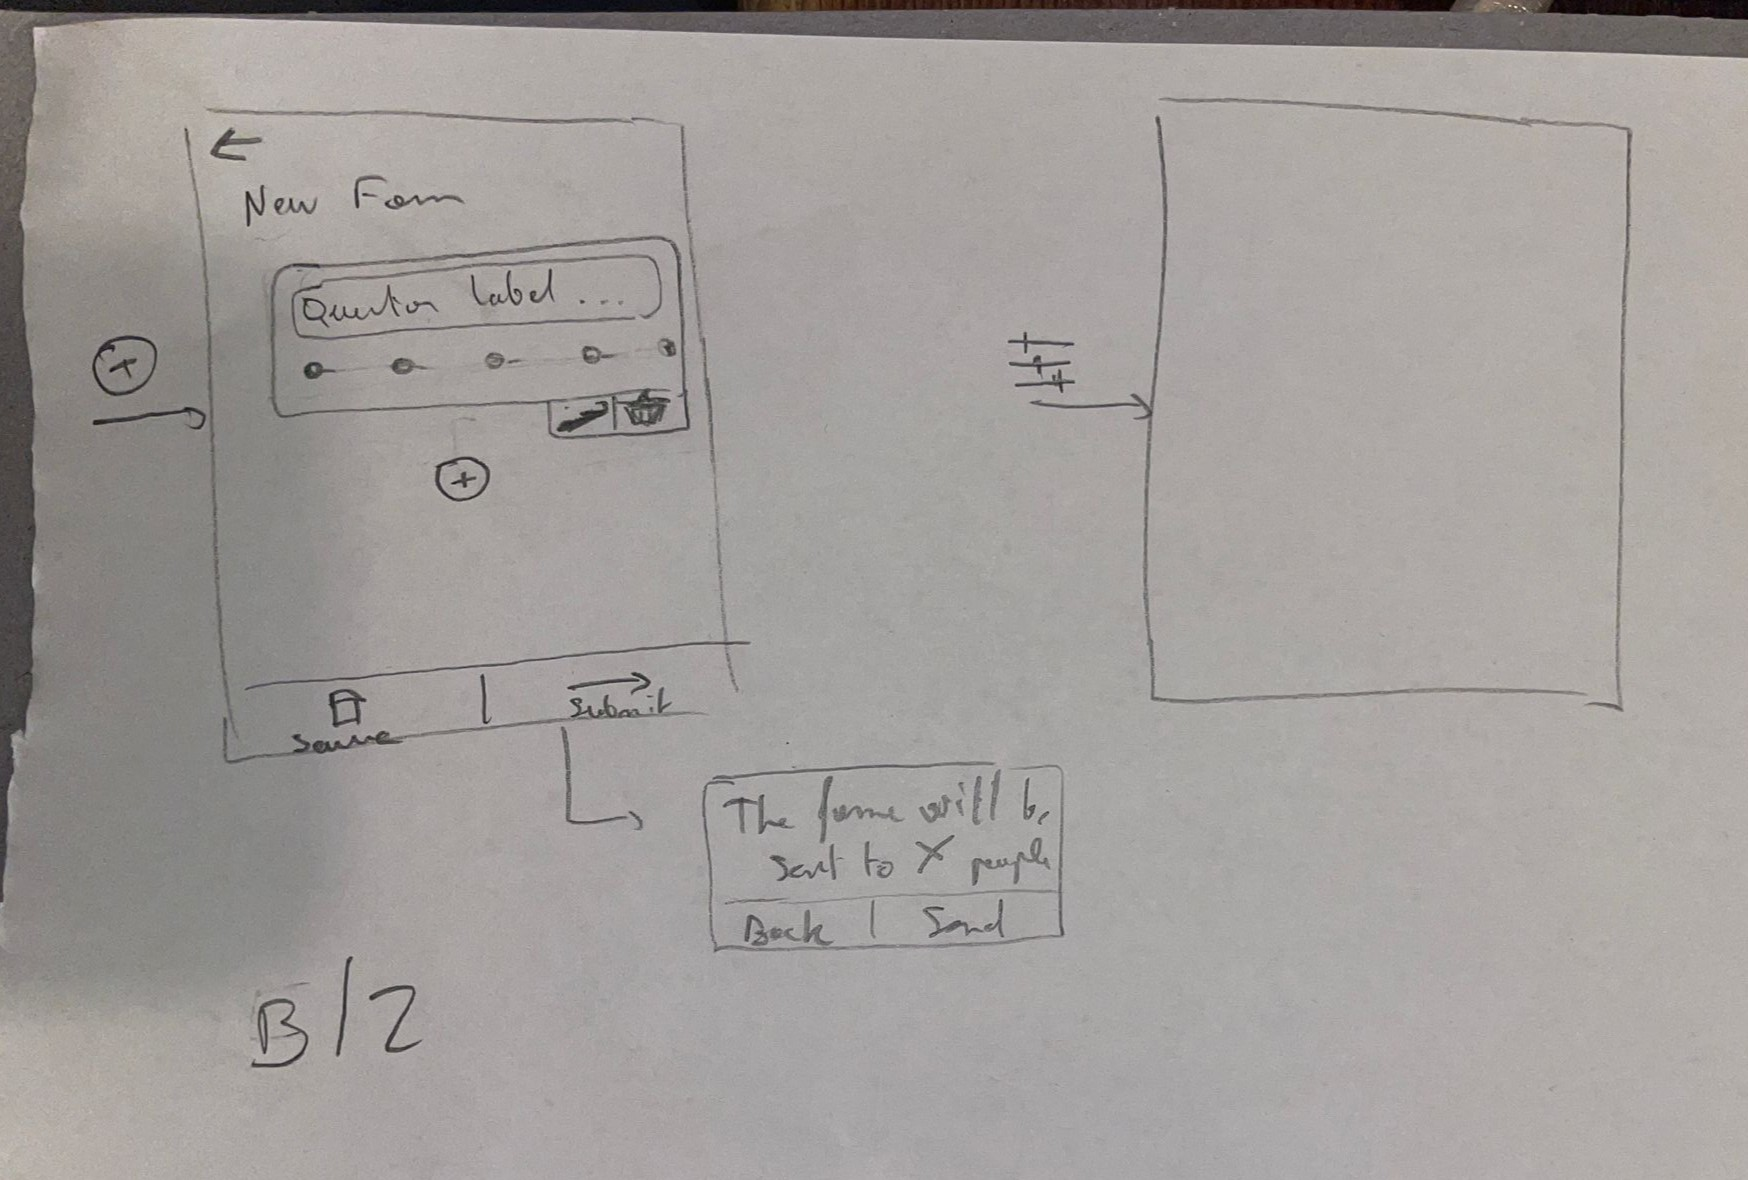
\includegraphics[width = \textwidth]{figures/B2.jpg}
    \caption{B only made minor adjustments in the second round and retained the structure. In addition, a screen for creating a form was added.}
\end{figure}

\begin{figure}[!h]
    \centering
    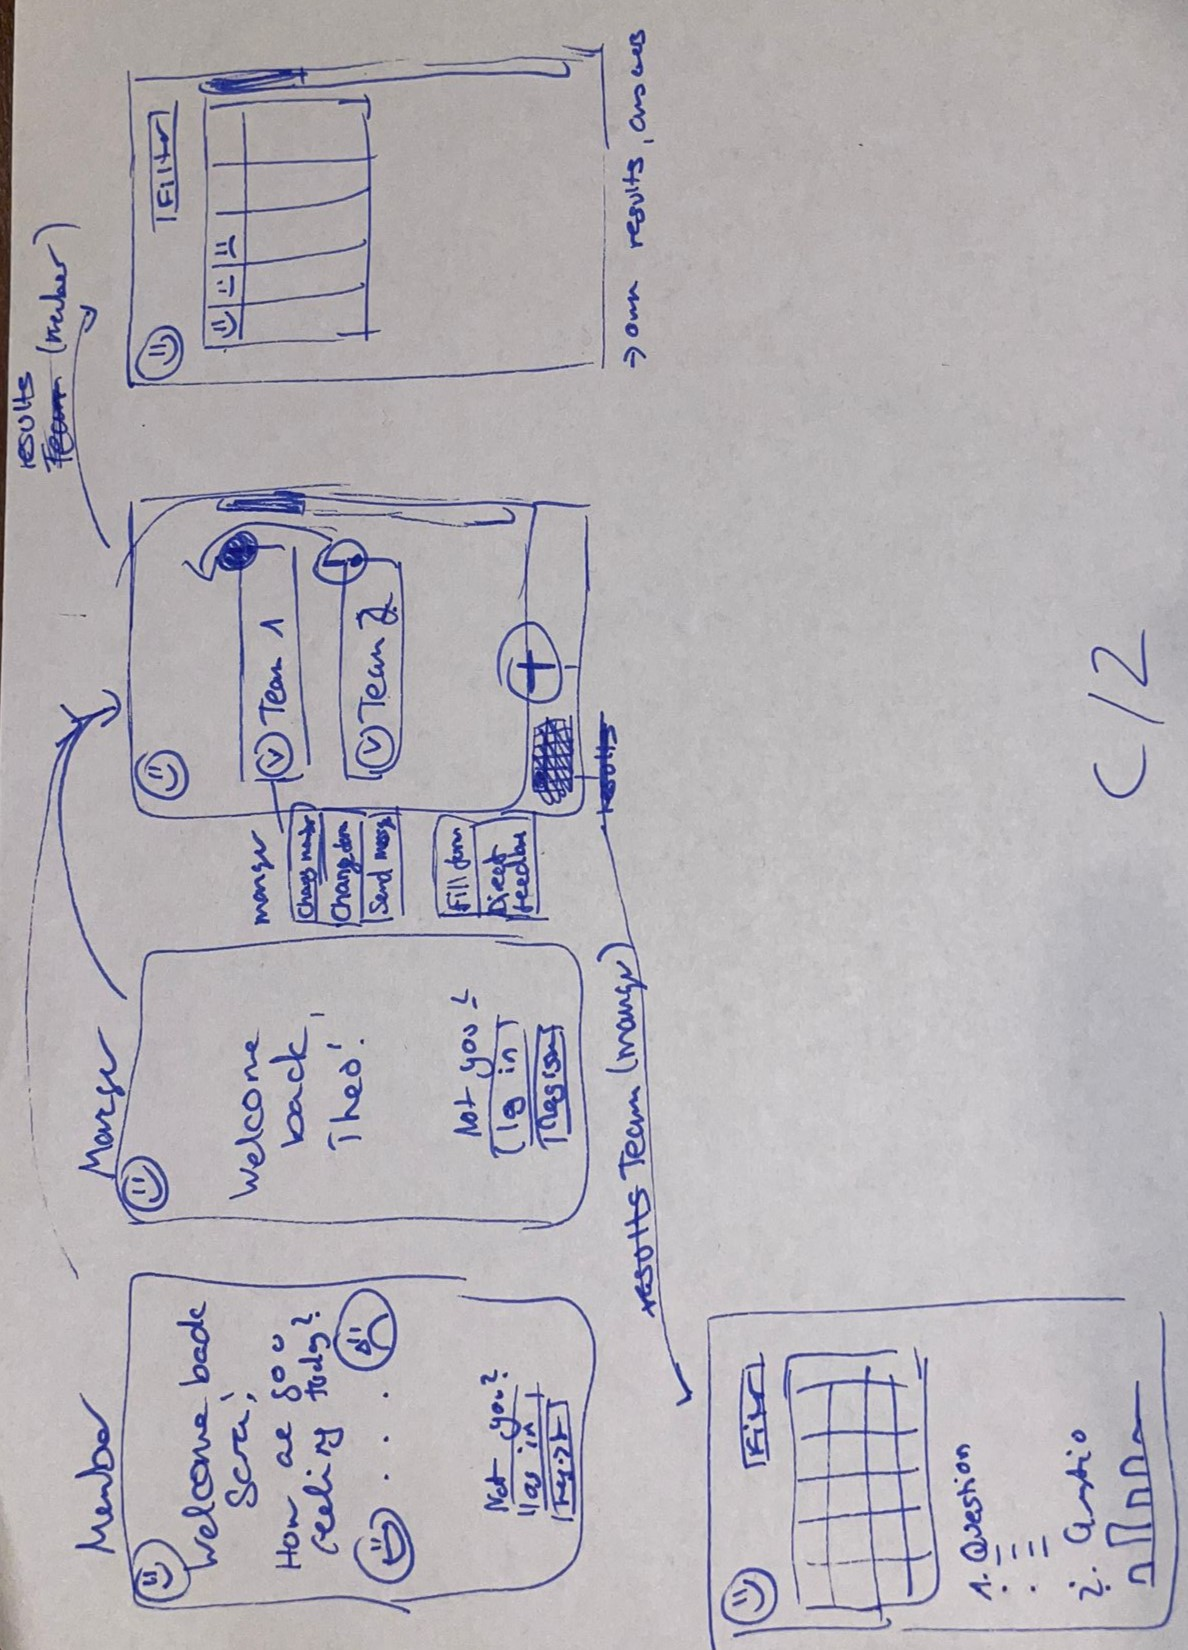
\includegraphics[width = \textwidth]{figures/C2.jpg}
    \caption{C has also adopted the team overview as the main screen and has retained almost everything else.}
\end{figure}

\begin{figure}[!h]
    \centering
    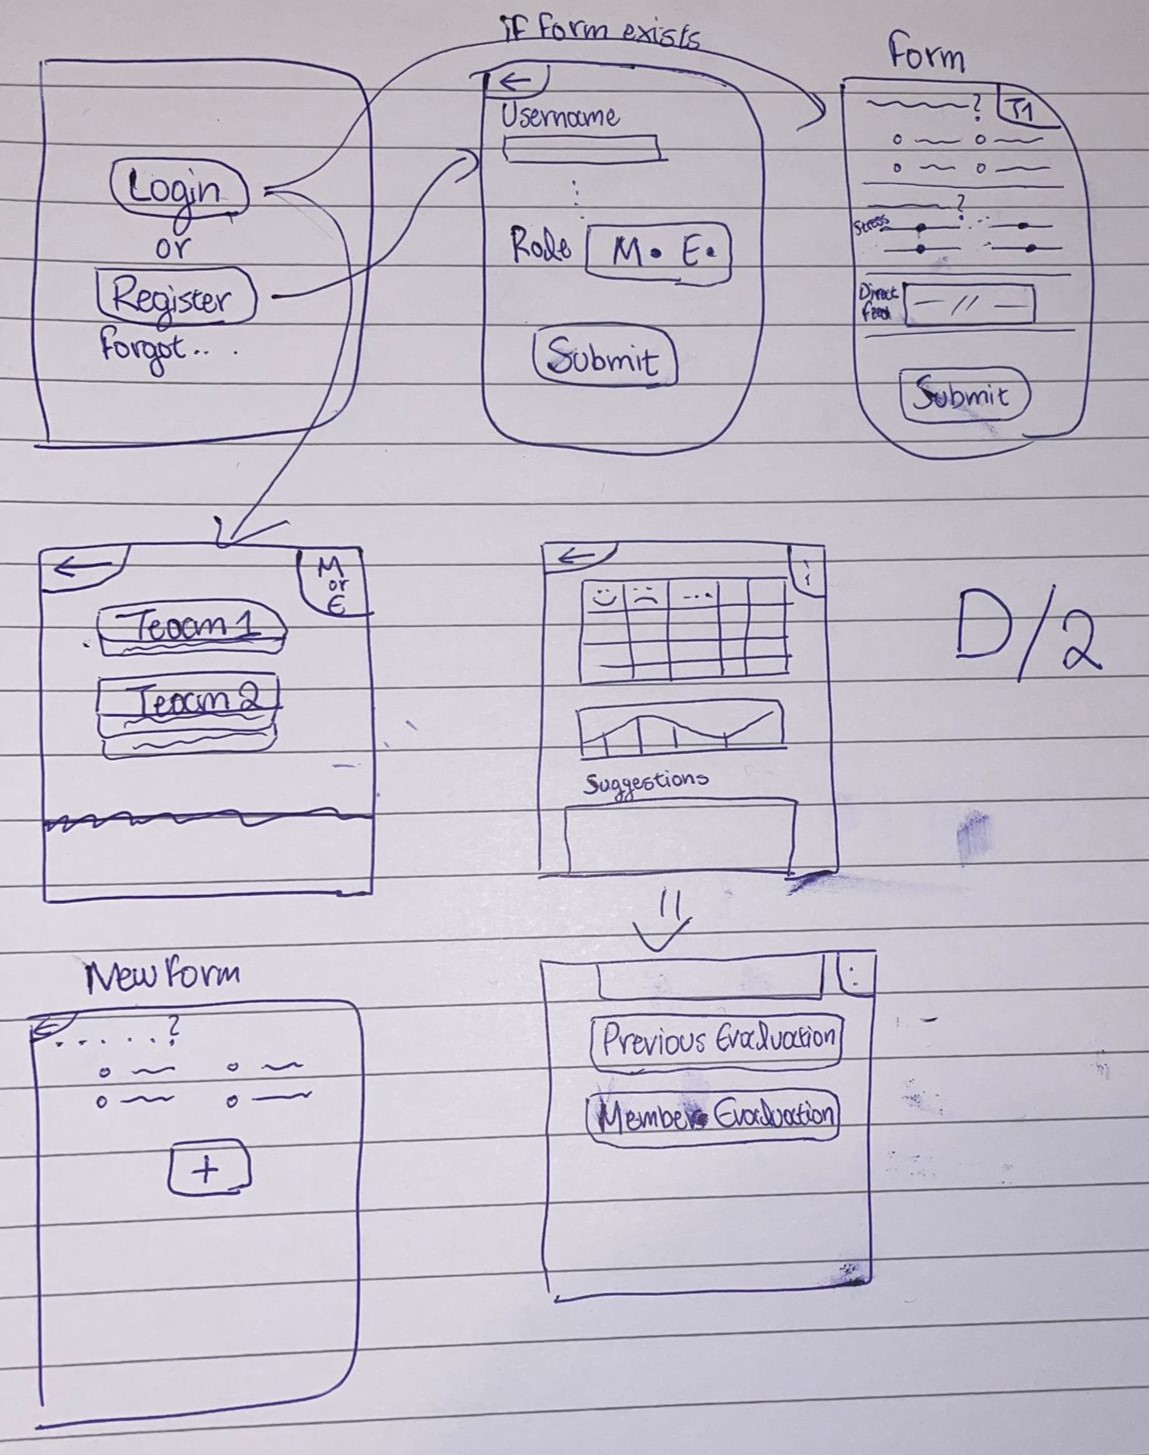
\includegraphics[width = \textwidth]{figures/D2.jpg}
    \caption{For D, in the second round design elements similar to those of the other team members were added and the team overview was adopted.}
\end{figure}

\clearpage


\subsection{Final Mockup}
The mockups show a few selected screens of our app. These include the login screen (1) with the daily mood query and the home screen (2; 5), on which all of the user's teams can be seen. The Team Leader and Team Member cases have been covered. There is also a screen on how we imagine the creation of a new survey (7) and the overview of the daily user (4) query.\\
After the user has answered the daily poll, he is redirected to the main screen. Here he has an overview of all his teams and can see when a new form is due. If he clicks on a team with a due form, he is forwarded directly to the form (not included here), otherwise he is taken to the team overview. 

\subsubsection{Alternative 1}
\begin{figure}[!h]
    \centering
    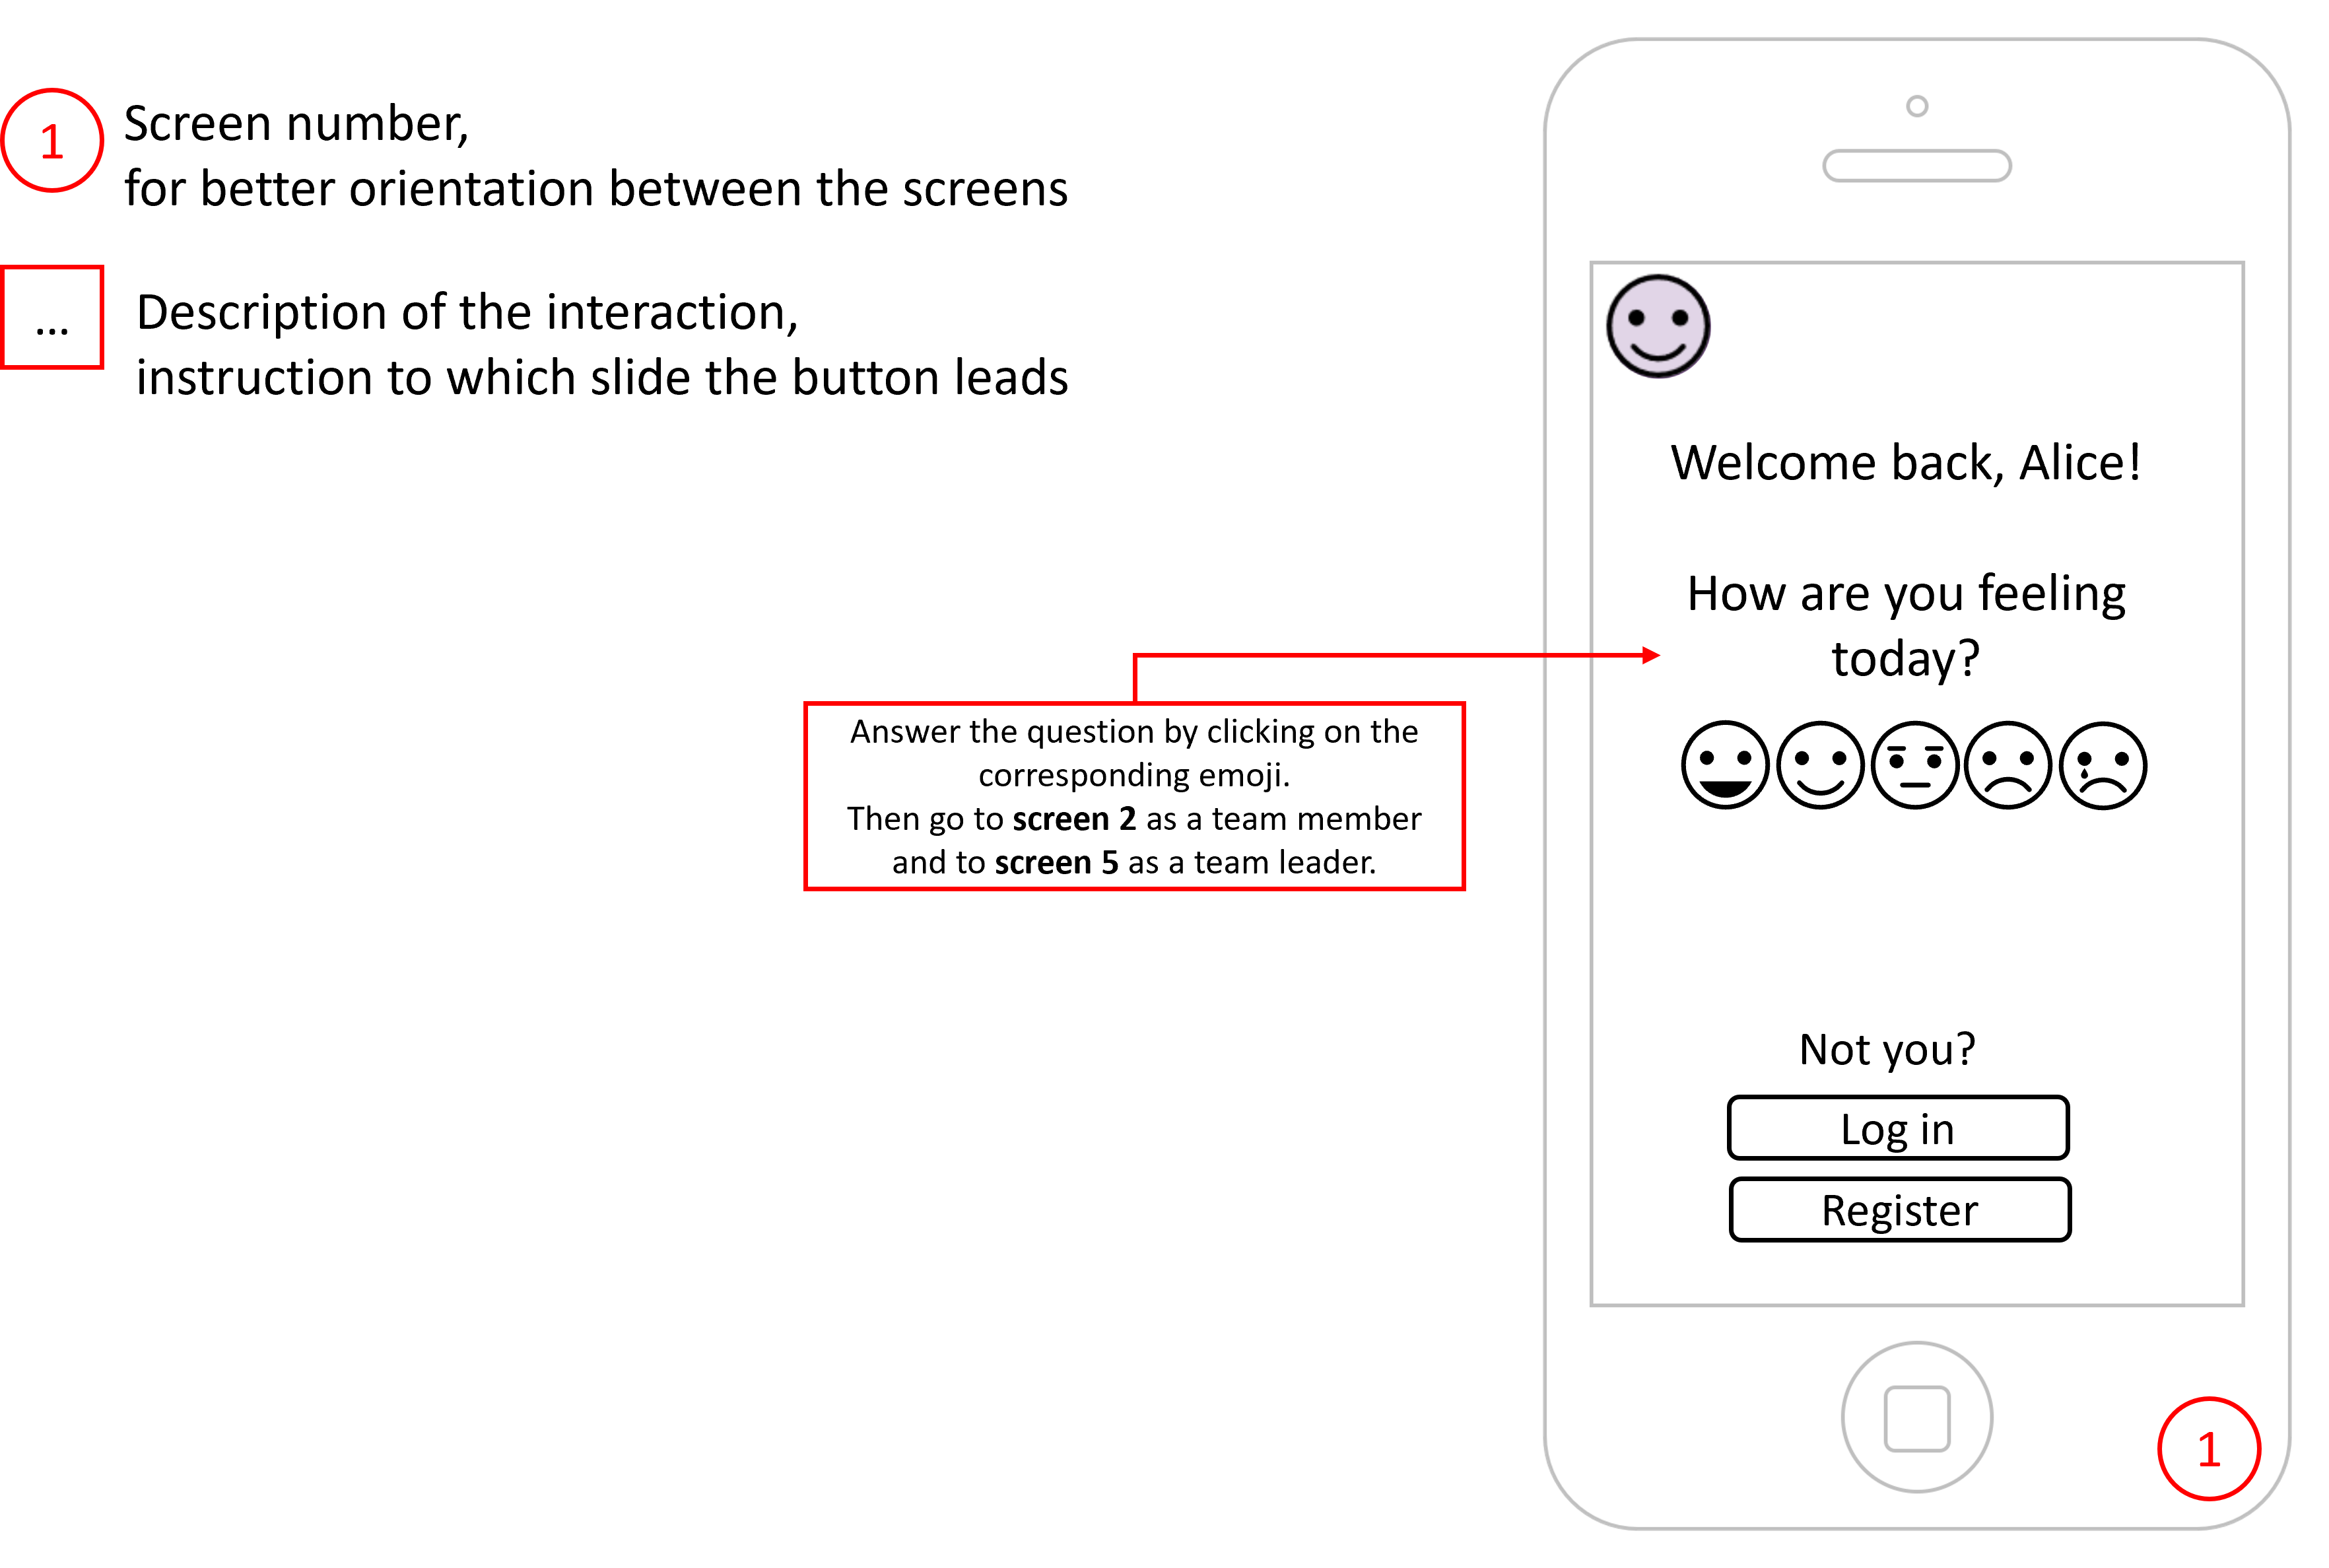
\includegraphics[width = \textwidth]{figures/Mock Up 1.png}
\end{figure}

\begin{figure}[!h]
    \centering
    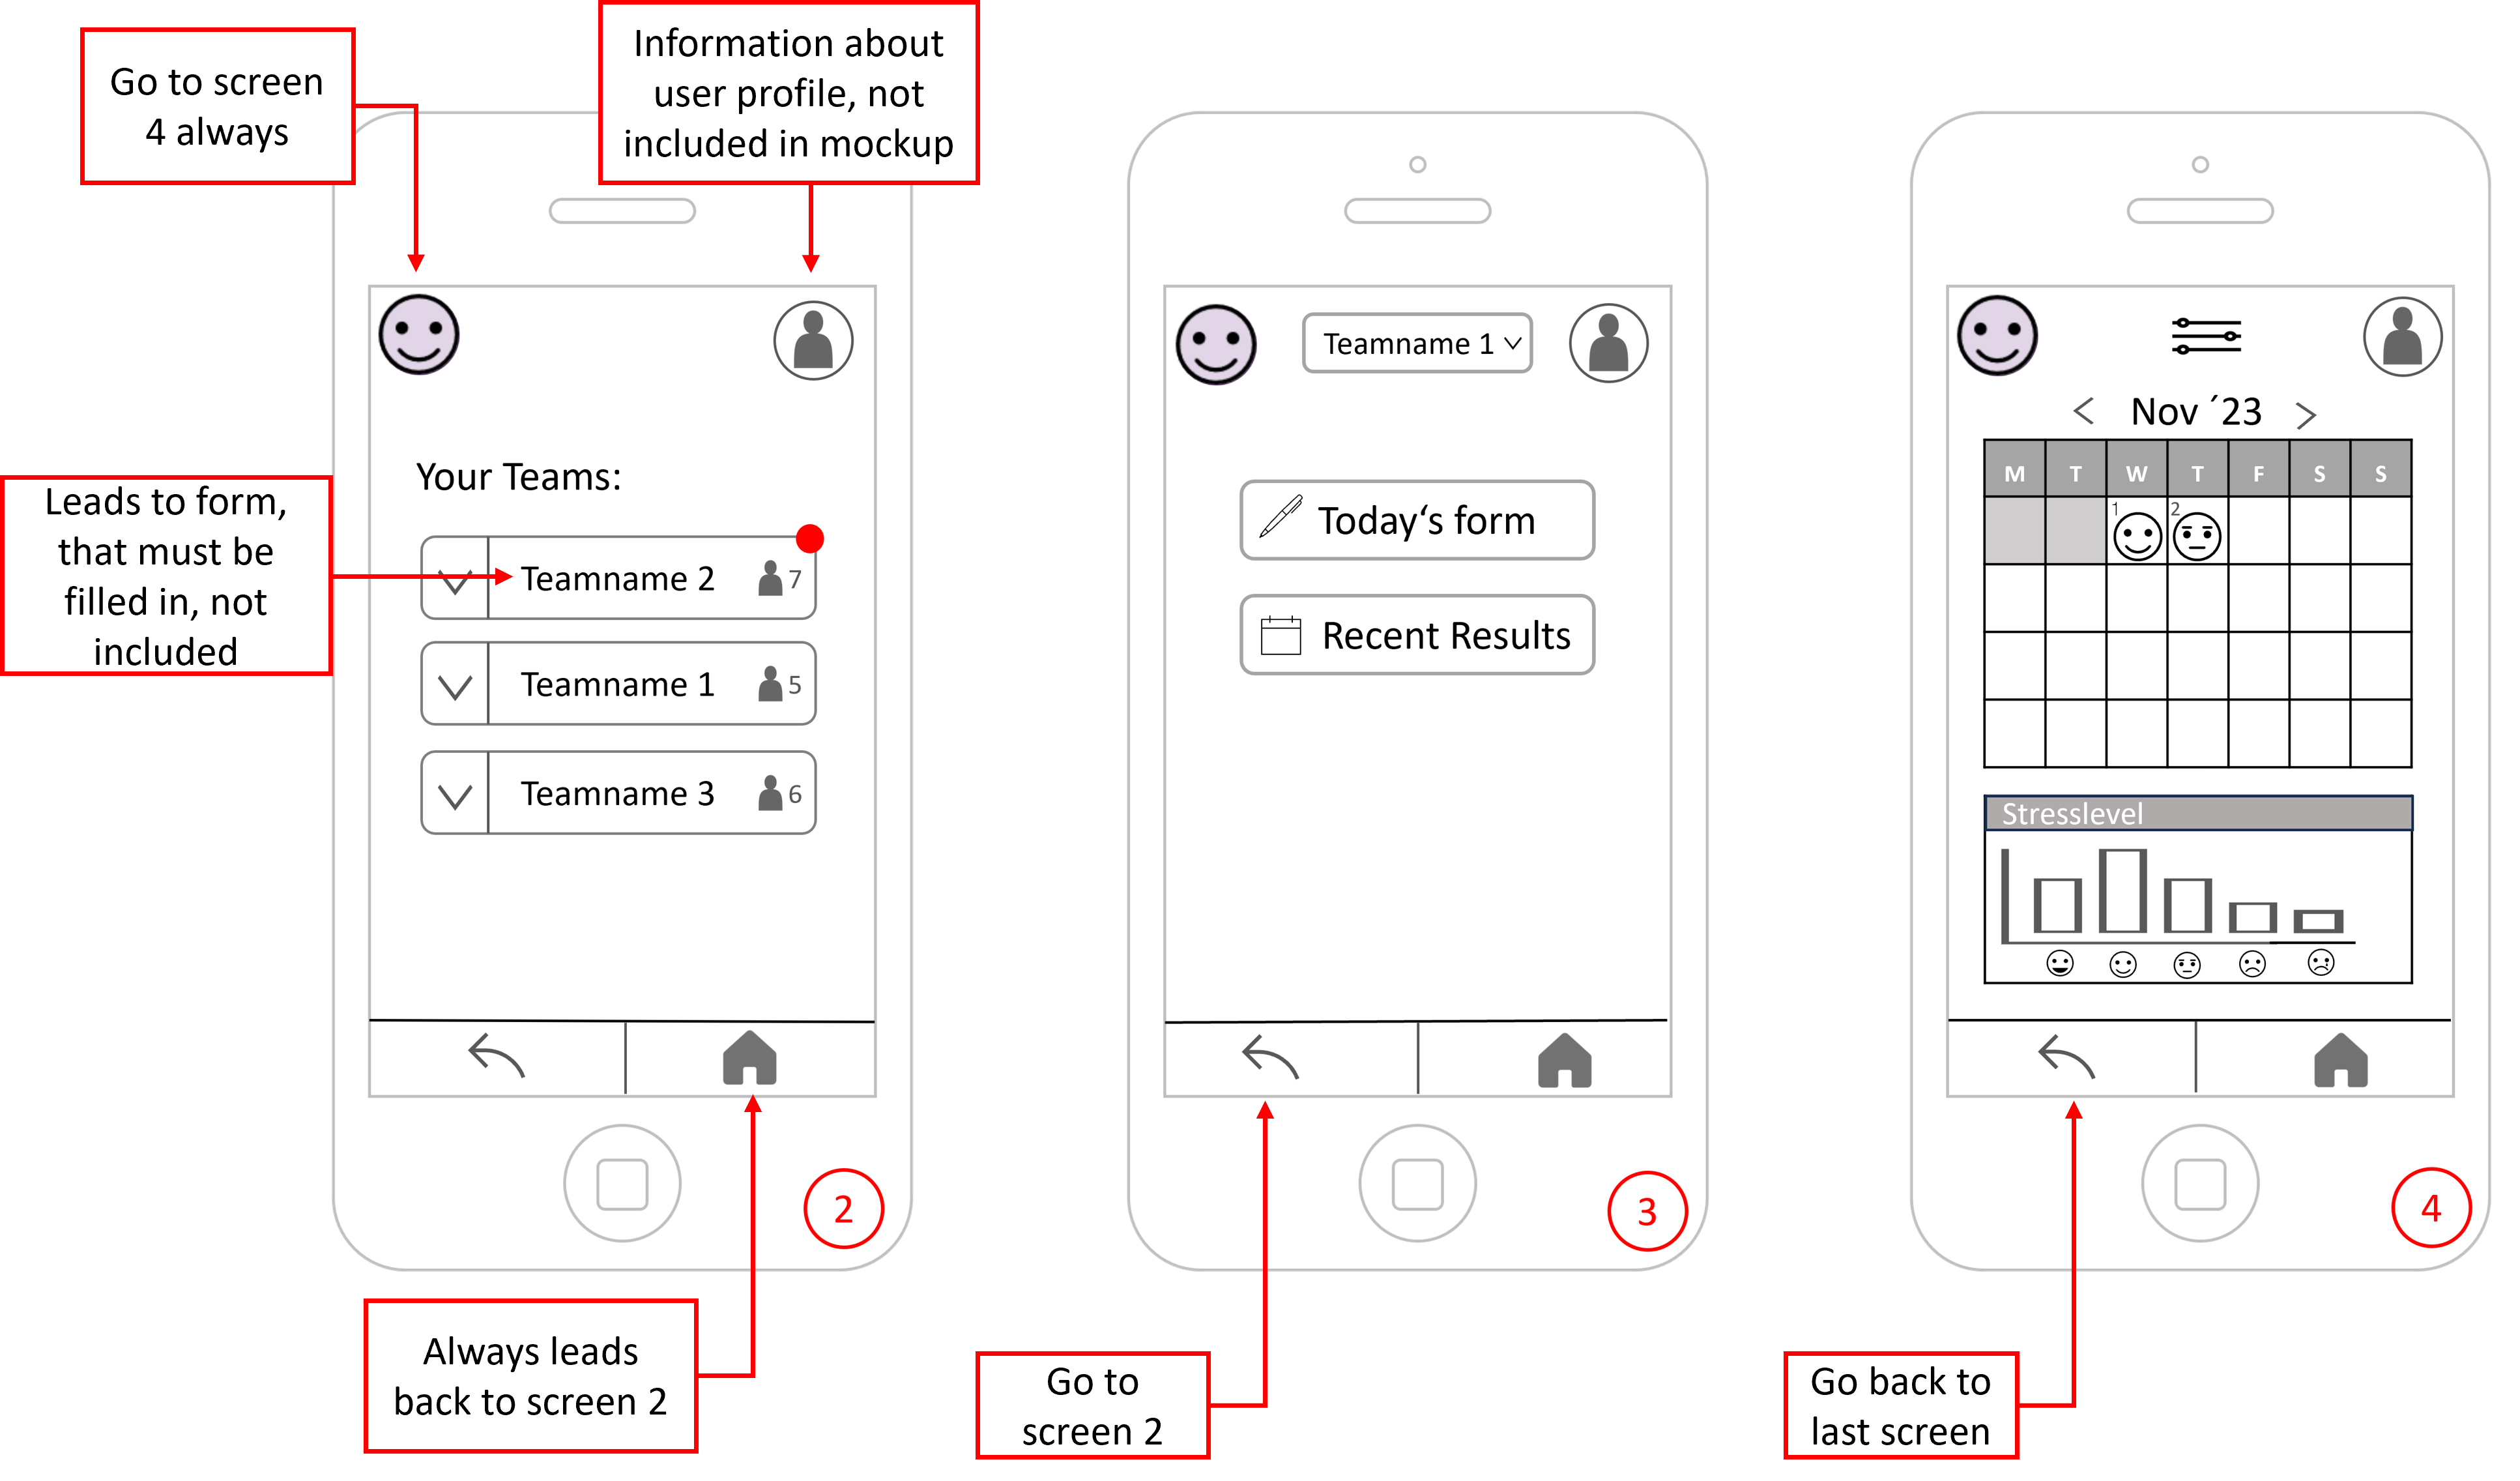
\includegraphics[width = \textwidth]{figures/Mock Up 2.png}
\end{figure}

\begin{figure}[!h]
    \centering
    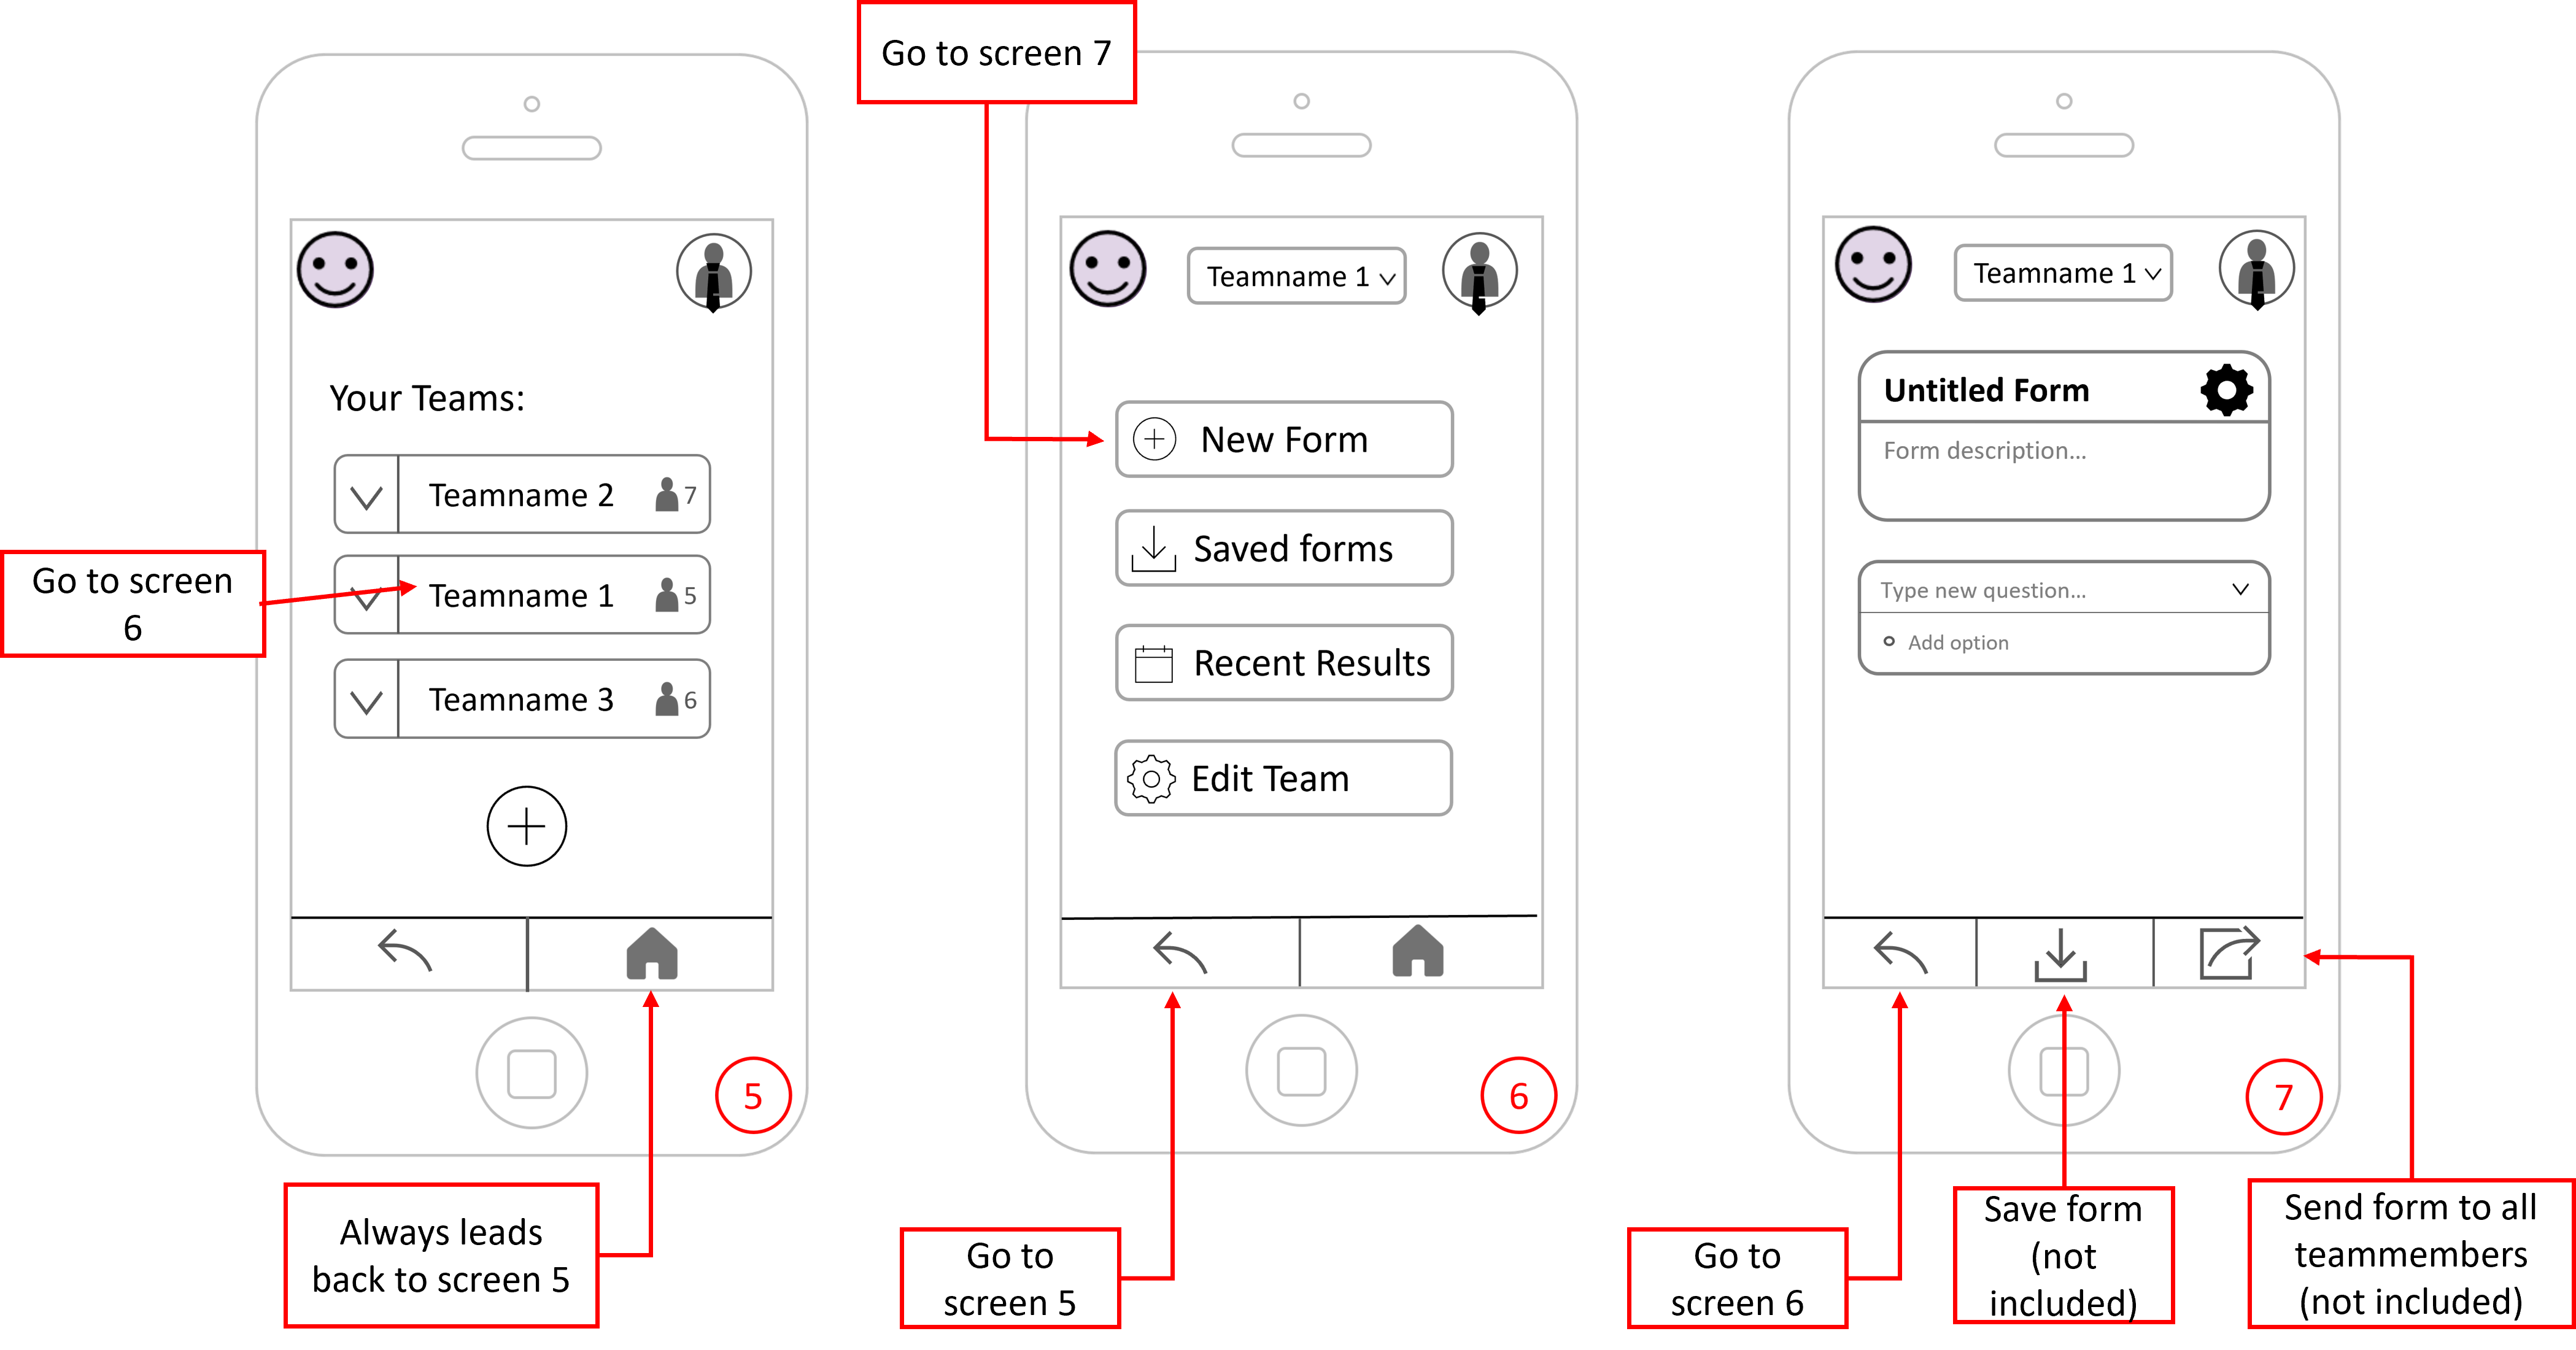
\includegraphics[width = \textwidth]{figures/Mock Up 3.png}
\end{figure}
\clearpage

\subsubsection{Alternative 2}

\begin{figure}[!h]
    \centering
    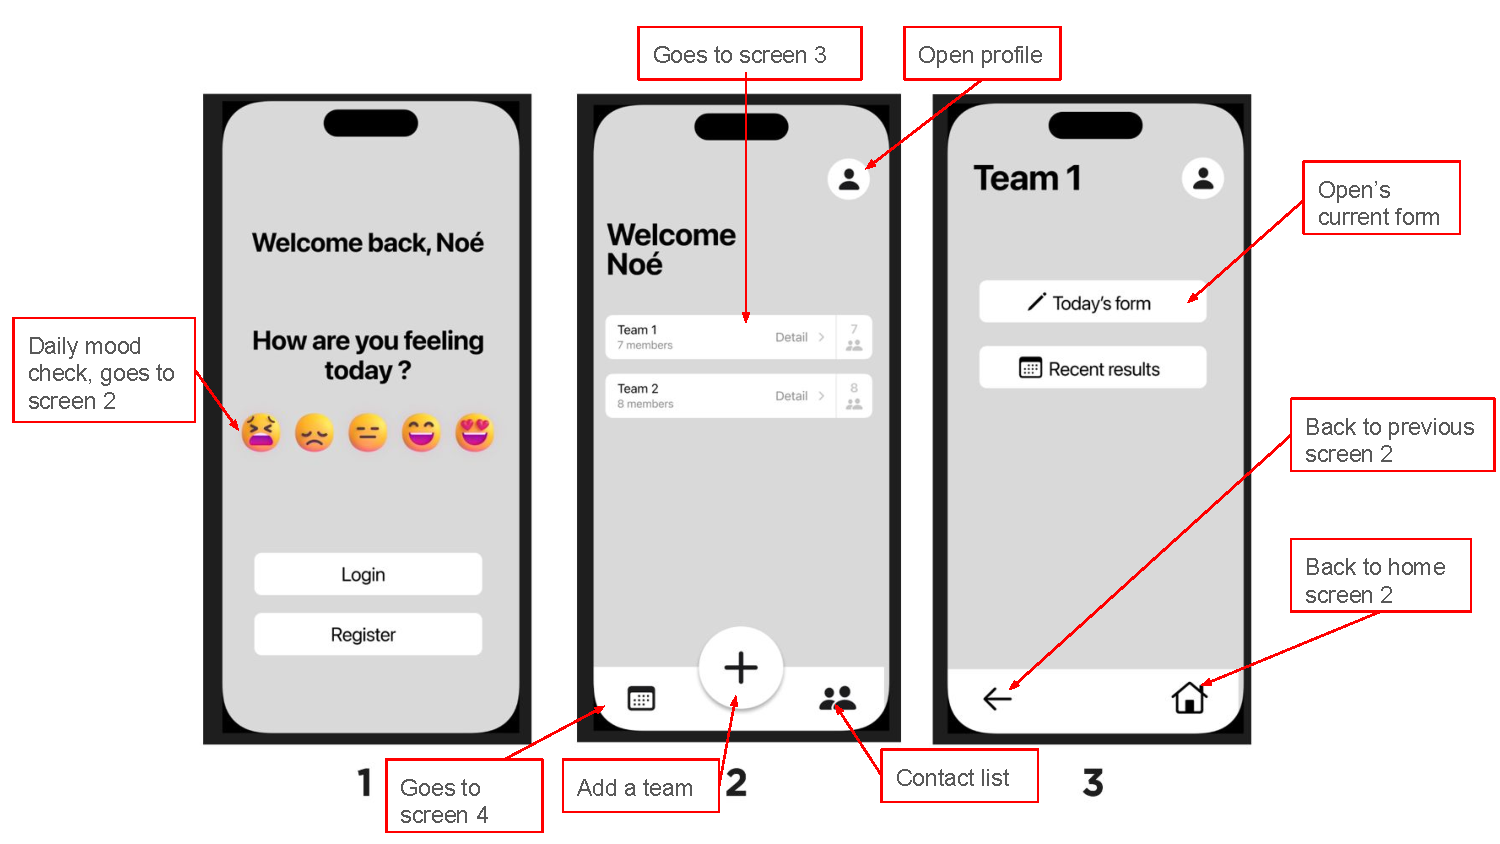
\includegraphics[width = \textwidth]{figures/figmaMockup-1.pdf}
\end{figure}
\begin{figure}[!h]
    \centering
    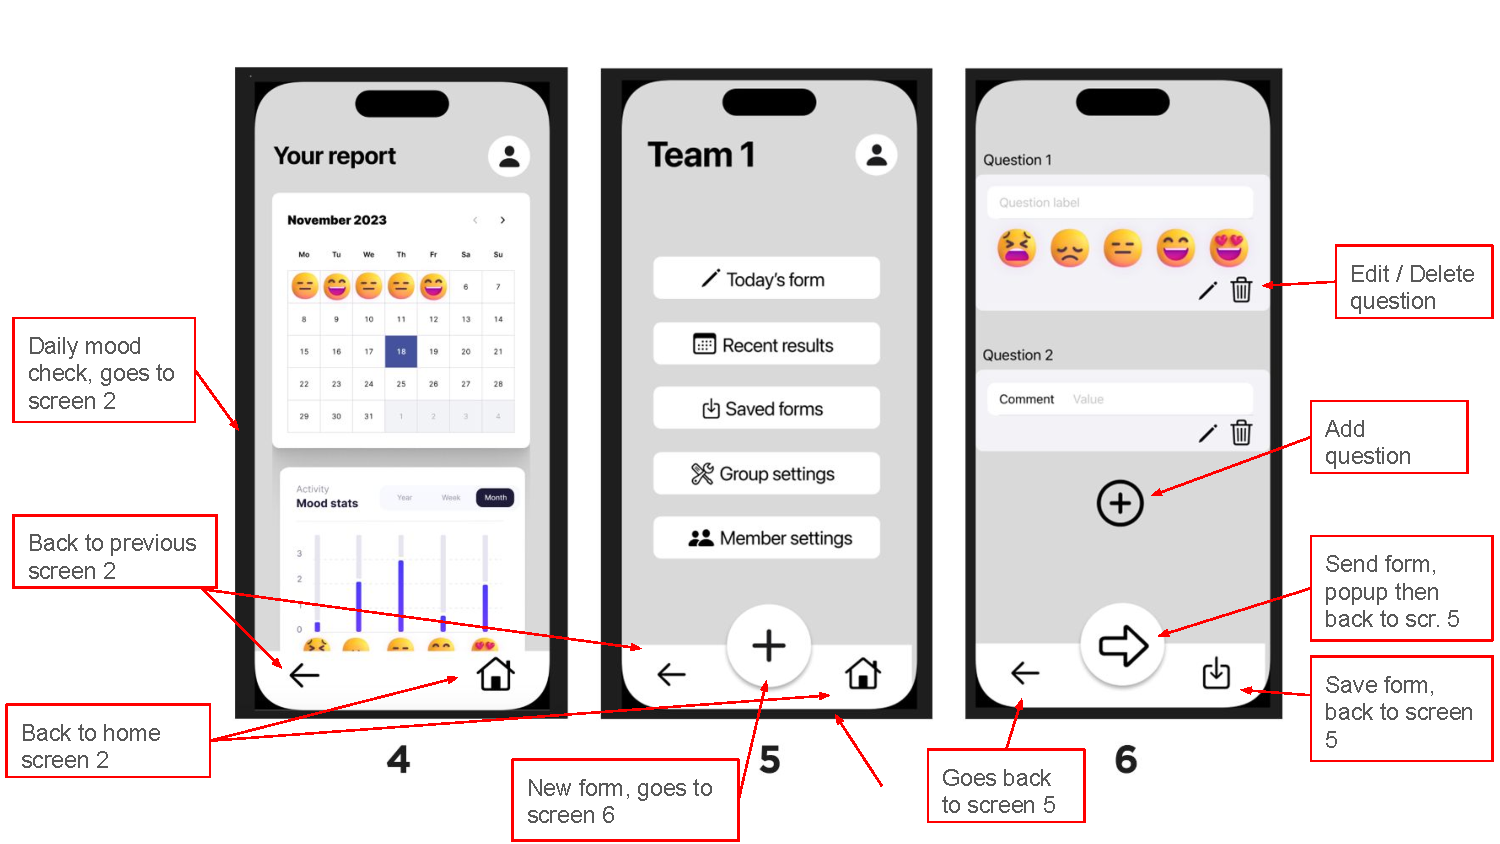
\includegraphics[width = \textwidth]{figures/figmaMockup-2.pdf}
\end{figure}



% --------------------
\printbibliography

% ==========================
% ==========================
% ==========================


\end{document}